\documentclass[twoside]{book}

% Packages required by doxygen
\usepackage{fixltx2e}
\usepackage{calc}
\usepackage{doxygen}
\usepackage[export]{adjustbox} % also loads graphicx
\usepackage{graphicx}
\usepackage[utf8]{inputenc}
\usepackage{makeidx}
\usepackage{multicol}
\usepackage{multirow}
\PassOptionsToPackage{warn}{textcomp}
\usepackage{textcomp}
\usepackage[nointegrals]{wasysym}
\usepackage[table]{xcolor}

% Font selection
\usepackage[T1]{fontenc}
\usepackage[scaled=.90]{helvet}
\usepackage{courier}
\usepackage{amssymb}
\usepackage{sectsty}
\renewcommand{\familydefault}{\sfdefault}
\allsectionsfont{%
  \fontseries{bc}\selectfont%
  \color{darkgray}%
}
\renewcommand{\DoxyLabelFont}{%
  \fontseries{bc}\selectfont%
  \color{darkgray}%
}
\newcommand{\+}{\discretionary{\mbox{\scriptsize$\hookleftarrow$}}{}{}}

% Page & text layout
\usepackage{geometry}
\geometry{%
  a4paper,%
  top=2.5cm,%
  bottom=2.5cm,%
  left=2.5cm,%
  right=2.5cm%
}
\tolerance=750
\hfuzz=15pt
\hbadness=750
\setlength{\emergencystretch}{15pt}
\setlength{\parindent}{0cm}
\setlength{\parskip}{3ex plus 2ex minus 2ex}
\makeatletter
\renewcommand{\paragraph}{%
  \@startsection{paragraph}{4}{0ex}{-1.0ex}{1.0ex}{%
    \normalfont\normalsize\bfseries\SS@parafont%
  }%
}
\renewcommand{\subparagraph}{%
  \@startsection{subparagraph}{5}{0ex}{-1.0ex}{1.0ex}{%
    \normalfont\normalsize\bfseries\SS@subparafont%
  }%
}
\makeatother

% Headers & footers
\usepackage{fancyhdr}
\pagestyle{fancyplain}
\fancyhead[LE]{\fancyplain{}{\bfseries\thepage}}
\fancyhead[CE]{\fancyplain{}{}}
\fancyhead[RE]{\fancyplain{}{\bfseries\leftmark}}
\fancyhead[LO]{\fancyplain{}{\bfseries\rightmark}}
\fancyhead[CO]{\fancyplain{}{}}
\fancyhead[RO]{\fancyplain{}{\bfseries\thepage}}
\fancyfoot[LE]{\fancyplain{}{}}
\fancyfoot[CE]{\fancyplain{}{}}
\fancyfoot[RE]{\fancyplain{}{\bfseries\scriptsize Generated by Doxygen }}
\fancyfoot[LO]{\fancyplain{}{\bfseries\scriptsize Generated by Doxygen }}
\fancyfoot[CO]{\fancyplain{}{}}
\fancyfoot[RO]{\fancyplain{}{}}
\renewcommand{\footrulewidth}{0.4pt}
\renewcommand{\chaptermark}[1]{%
  \markboth{#1}{}%
}
\renewcommand{\sectionmark}[1]{%
  \markright{\thesection\ #1}%
}

% Indices & bibliography
\usepackage{natbib}
\usepackage[titles]{tocloft}
\setcounter{tocdepth}{3}
\setcounter{secnumdepth}{5}
\makeindex

% Hyperlinks (required, but should be loaded last)
\usepackage{ifpdf}
\ifpdf
  \usepackage[pdftex,pagebackref=true]{hyperref}
\else
  \usepackage[ps2pdf,pagebackref=true]{hyperref}
\fi
\hypersetup{%
  colorlinks=true,%
  linkcolor=blue,%
  citecolor=blue,%
  unicode%
}

% Custom commands
\newcommand{\clearemptydoublepage}{%
  \newpage{\pagestyle{empty}\cleardoublepage}%
}

\usepackage{caption}
\captionsetup{labelsep=space,justification=centering,font={bf},singlelinecheck=off,skip=4pt,position=top}

%===== C O N T E N T S =====

\begin{document}

% Titlepage & ToC
\hypersetup{pageanchor=false,
             bookmarksnumbered=true,
             pdfencoding=unicode
            }
\pagenumbering{roman}
\begin{titlepage}
\vspace*{7cm}
\begin{center}%
{\Large function\+\_\+traits \\[1ex]\large 0.\+1 }\\
\vspace*{1cm}
{\large Generated by Doxygen 1.8.11}\\
\end{center}
\end{titlepage}
\clearemptydoublepage
\tableofcontents
\clearemptydoublepage
\pagenumbering{arabic}
\hypersetup{pageanchor=true}

%--- Begin generated contents ---
\chapter{function\+\_\+traits}
\label{index}\hypertarget{index}{}\subsubsection*{Example\+:}


\begin{DoxyCode}
1 \{C++\}
2 
3 #include <type\_traits>
4 #include <iostream>
5 #include <iomanip>
6 
7 #include <function\_traits.hpp>
8 
9 using namespace std;
10 using namespace fn\_traits;
11 
12 int myFunction( int, float ) \{
13 
14 \}
15 
16 int main() \{
17     typedef function\_traits<decltype( myFunction )> traits;
18 
19     cout << boolalpha << is\_same<int, typename traits::template arg<0>::type>::value << endl; //true
20 
21     auto cb = []() -> double \{
22         return 10.0;
23     \};
24 
25     cout << boolalpha << is\_same<double, typename function\_traits<decltype( cb )>::result\_type>::value <<
       endl; //true
26 
27     return 0;
28 \}
\end{DoxyCode}


\subsubsection*{A\+PI}

\paragraph*{\href{https://novacrazy.github.io/function_traits/html/index.html}{\tt Click here for Doxygen generated documentation}}

All of these are within the namespace {\ttfamily \hyperlink{namespacefn__traits}{fn\+\_\+traits}}.

\paragraph*{{\ttfamily function\+\_\+traits$<$Functor$>$\+::arity}}

Integer value representing the number of parameters in the given Functor

\paragraph*{{\ttfamily function\+\_\+traits$<$Functor$>$\+::result\+\_\+type}}

\subparagraph*{alias\+: {\ttfamily function\+\_\+traits$<$Functor$>$\+::return\+\_\+type}}

The return/result type of the Functor

\paragraph*{{\ttfamily function\+\_\+traits$<$Functor$>$\+::function\+\_\+type}}

A simplified version of Functor

\paragraph*{{\ttfamily function\+\_\+traits$<$Functor$>$\+::template arg$<$N$>$\+::type}}

Access the type of argument {\ttfamily N}

\paragraph*{{\ttfamily function\+\_\+traits$<$Functor$>$\+::tuple\+\_\+type}}

Shortcut for {\ttfamily std\+::tuple$<$Args...$>$} where {\ttfamily Args...} are the arguments of the Functor given. 
\chapter{Namespace Index}
\section{Namespace List}
Here is a list of all namespaces with brief descriptions\+:\begin{DoxyCompactList}
\item\contentsline{section}{\hyperlink{namespacefn__traits}{fn\+\_\+traits} }{\pageref{dd/df9/namespacefn__traits}}{}
\end{DoxyCompactList}

\chapter{Hierarchical Index}
\section{Class Hierarchy}
This inheritance list is sorted roughly, but not completely, alphabetically\+:\begin{DoxyCompactList}
\item \contentsline{section}{fn\+\_\+traits\+:\+:function\+\_\+traits$<$ R(Args...)$>$\+:\+:arg$<$ i $>$}{\pageref{structfn__traits_1_1function__traits_3_01_r_07_args_8_8_8_08_4}}{}
\item \contentsline{section}{fn\+\_\+traits\+:\+:function\+\_\+traits$<$ Functor $>$}{\pageref{structfn__traits_1_1function__traits}}{}
\begin{DoxyCompactList}
\item \contentsline{section}{fn\+\_\+traits\+:\+:function\+\_\+traits$<$ std\+:\+:function$<$ Functor $>$ $>$}{\pageref{structfn__traits_1_1function__traits_3_01std_1_1function_3_01_functor_01_4_01_4}}{}
\end{DoxyCompactList}
\item \contentsline{section}{fn\+\_\+traits\+:\+:function\+\_\+traits$<$ R(Args...)$>$}{\pageref{structfn__traits_1_1function__traits_3_01_r_07_args_8_8_8_08_4}}{}
\begin{DoxyCompactList}
\item \contentsline{section}{fn\+\_\+traits\+:\+:function\+\_\+traits$<$ R($\ast$)(Args...)$>$}{\pageref{structfn__traits_1_1function__traits_3_01_r_07_5_08_07_args_8_8_8_08_4}}{}
\item \contentsline{section}{fn\+\_\+traits\+:\+:function\+\_\+traits$<$ R(C\+:\+:$\ast$)(Args...) const $>$}{\pageref{structfn__traits_1_1function__traits_3_01_r_07_c_1_1_5_08_07_args_8_8_8_08_01const_01_01_4}}{}
\item \contentsline{section}{fn\+\_\+traits\+:\+:function\+\_\+traits$<$ R(C\+:\+:$\ast$)(Args...) const volatile $>$}{\pageref{structfn__traits_1_1function__traits_3_01_r_07_c_1_1_5_08_07_args_8_8_8_08_01const_01volatile_01_4}}{}
\item \contentsline{section}{fn\+\_\+traits\+:\+:function\+\_\+traits$<$ R(C\+:\+:$\ast$)(Args...) volatile $>$}{\pageref{structfn__traits_1_1function__traits_3_01_r_07_c_1_1_5_08_07_args_8_8_8_08_01volatile_01_4}}{}
\item \contentsline{section}{fn\+\_\+traits\+:\+:function\+\_\+traits$<$ R(C\+:\+:$\ast$)(Args...)$>$}{\pageref{structfn__traits_1_1function__traits_3_01_r_07_c_1_1_5_08_07_args_8_8_8_08_4}}{}
\end{DoxyCompactList}
\item \contentsline{section}{fn\+\_\+traits\+:\+:function\+\_\+traits$<$ T $>$}{\pageref{structfn__traits_1_1function__traits}}{}
\begin{DoxyCompactList}
\item \contentsline{section}{fn\+\_\+traits\+:\+:function\+\_\+traits$<$ const T \& $>$}{\pageref{structfn__traits_1_1function__traits_3_01const_01_t_01_6_01_4}}{}
\item \contentsline{section}{fn\+\_\+traits\+:\+:function\+\_\+traits$<$ const T \&\& $>$}{\pageref{structfn__traits_1_1function__traits_3_01const_01_t_01_6_6_01_4}}{}
\item \contentsline{section}{fn\+\_\+traits\+:\+:function\+\_\+traits$<$ const volatile T \& $>$}{\pageref{structfn__traits_1_1function__traits_3_01const_01volatile_01_t_01_6_01_4}}{}
\item \contentsline{section}{fn\+\_\+traits\+:\+:function\+\_\+traits$<$ const volatile T \&\& $>$}{\pageref{structfn__traits_1_1function__traits_3_01const_01volatile_01_t_01_6_6_01_4}}{}
\item \contentsline{section}{fn\+\_\+traits\+:\+:function\+\_\+traits$<$ T \& $>$}{\pageref{structfn__traits_1_1function__traits_3_01_t_01_6_01_4}}{}
\item \contentsline{section}{fn\+\_\+traits\+:\+:function\+\_\+traits$<$ T \&\& $>$}{\pageref{structfn__traits_1_1function__traits_3_01_t_01_6_6_01_4}}{}
\item \contentsline{section}{fn\+\_\+traits\+:\+:function\+\_\+traits$<$ volatile T \& $>$}{\pageref{structfn__traits_1_1function__traits_3_01volatile_01_t_01_6_01_4}}{}
\item \contentsline{section}{fn\+\_\+traits\+:\+:function\+\_\+traits$<$ volatile T \&\& $>$}{\pageref{structfn__traits_1_1function__traits_3_01volatile_01_t_01_6_6_01_4}}{}
\end{DoxyCompactList}
\end{DoxyCompactList}

\chapter{Class Index}
\section{Class List}
Here are the classes, structs, unions and interfaces with brief descriptions\+:\begin{DoxyCompactList}
\item\contentsline{section}{\hyperlink{structfn__traits_1_1function__traits}{fn\+\_\+traits\+::function\+\_\+traits$<$ Functor $>$} }{\pageref{d8/ddb/structfn__traits_1_1function__traits}}{}
\item\contentsline{section}{\hyperlink{structfn__traits_1_1function__traits_3_01const_01_t_01_6_01_4}{fn\+\_\+traits\+::function\+\_\+traits$<$ const T \& $>$} }{\pageref{df/d00/structfn__traits_1_1function__traits_3_01const_01_t_01_6_01_4}}{}
\item\contentsline{section}{\hyperlink{structfn__traits_1_1function__traits_3_01const_01_t_01_6_6_01_4}{fn\+\_\+traits\+::function\+\_\+traits$<$ const T \&\& $>$} }{\pageref{d5/dad/structfn__traits_1_1function__traits_3_01const_01_t_01_6_6_01_4}}{}
\item\contentsline{section}{\hyperlink{structfn__traits_1_1function__traits_3_01const_01volatile_01_t_01_6_01_4}{fn\+\_\+traits\+::function\+\_\+traits$<$ const volatile T \& $>$} }{\pageref{d3/d03/structfn__traits_1_1function__traits_3_01const_01volatile_01_t_01_6_01_4}}{}
\item\contentsline{section}{\hyperlink{structfn__traits_1_1function__traits_3_01const_01volatile_01_t_01_6_6_01_4}{fn\+\_\+traits\+::function\+\_\+traits$<$ const volatile T \&\& $>$} }{\pageref{d6/daa/structfn__traits_1_1function__traits_3_01const_01volatile_01_t_01_6_6_01_4}}{}
\item\contentsline{section}{\hyperlink{structfn__traits_1_1function__traits_3_01_r_07_5_08_07_args_8_8_8_08_4}{fn\+\_\+traits\+::function\+\_\+traits$<$ R($\ast$)(\+Args...)$>$} }{\pageref{d7/d49/structfn__traits_1_1function__traits_3_01_r_07_5_08_07_args_8_8_8_08_4}}{}
\item\contentsline{section}{\hyperlink{structfn__traits_1_1function__traits_3_01_r_07_args_8_8_8_08_4}{fn\+\_\+traits\+::function\+\_\+traits$<$ R(\+Args...)$>$} }{\pageref{d7/d49/structfn__traits_1_1function__traits_3_01_r_07_args_8_8_8_08_4}}{}
\item\contentsline{section}{\hyperlink{structfn__traits_1_1function__traits_3_01_r_07_c_1_1_5_08_07_args_8_8_8_08_01const_01_01_4}{fn\+\_\+traits\+::function\+\_\+traits$<$ R(\+C\+::$\ast$)(\+Args...) const  $>$} }{\pageref{db/df0/structfn__traits_1_1function__traits_3_01_r_07_c_1_1_5_08_07_args_8_8_8_08_01const_01_01_4}}{}
\item\contentsline{section}{\hyperlink{structfn__traits_1_1function__traits_3_01_r_07_c_1_1_5_08_07_args_8_8_8_08_01const_01volatile_01_4}{fn\+\_\+traits\+::function\+\_\+traits$<$ R(\+C\+::$\ast$)(\+Args...) const volatile $>$} }{\pageref{d9/d43/structfn__traits_1_1function__traits_3_01_r_07_c_1_1_5_08_07_args_8_8_8_08_01const_01volatile_01_4}}{}
\item\contentsline{section}{\hyperlink{structfn__traits_1_1function__traits_3_01_r_07_c_1_1_5_08_07_args_8_8_8_08_01volatile_01_4}{fn\+\_\+traits\+::function\+\_\+traits$<$ R(\+C\+::$\ast$)(\+Args...) volatile $>$} }{\pageref{d3/db9/structfn__traits_1_1function__traits_3_01_r_07_c_1_1_5_08_07_args_8_8_8_08_01volatile_01_4}}{}
\item\contentsline{section}{\hyperlink{structfn__traits_1_1function__traits_3_01_r_07_c_1_1_5_08_07_args_8_8_8_08_4}{fn\+\_\+traits\+::function\+\_\+traits$<$ R(\+C\+::$\ast$)(\+Args...)$>$} }{\pageref{d9/da0/structfn__traits_1_1function__traits_3_01_r_07_c_1_1_5_08_07_args_8_8_8_08_4}}{}
\item\contentsline{section}{\hyperlink{structfn__traits_1_1function__traits_3_01std_1_1function_3_01_functor_01_4_01_4}{fn\+\_\+traits\+::function\+\_\+traits$<$ std\+::function$<$ Functor $>$ $>$} }{\pageref{da/d97/structfn__traits_1_1function__traits_3_01std_1_1function_3_01_functor_01_4_01_4}}{}
\item\contentsline{section}{\hyperlink{structfn__traits_1_1function__traits_3_01_t_01_6_01_4}{fn\+\_\+traits\+::function\+\_\+traits$<$ T \& $>$} }{\pageref{d8/d39/structfn__traits_1_1function__traits_3_01_t_01_6_01_4}}{}
\item\contentsline{section}{\hyperlink{structfn__traits_1_1function__traits_3_01_t_01_6_6_01_4}{fn\+\_\+traits\+::function\+\_\+traits$<$ T \&\& $>$} }{\pageref{d9/dac/structfn__traits_1_1function__traits_3_01_t_01_6_6_01_4}}{}
\item\contentsline{section}{\hyperlink{structfn__traits_1_1function__traits_3_01volatile_01_t_01_6_01_4}{fn\+\_\+traits\+::function\+\_\+traits$<$ volatile T \& $>$} }{\pageref{d0/dc4/structfn__traits_1_1function__traits_3_01volatile_01_t_01_6_01_4}}{}
\item\contentsline{section}{\hyperlink{structfn__traits_1_1function__traits_3_01volatile_01_t_01_6_6_01_4}{fn\+\_\+traits\+::function\+\_\+traits$<$ volatile T \&\& $>$} }{\pageref{d1/ddf/structfn__traits_1_1function__traits_3_01volatile_01_t_01_6_6_01_4}}{}
\end{DoxyCompactList}

\chapter{File Index}
\section{File List}
Here is a list of all files with brief descriptions\+:\begin{DoxyCompactList}
\item\contentsline{section}{include/\hyperlink{function__traits_8hpp}{function\+\_\+traits.\+hpp} }{\pageref{d0/d52/function__traits_8hpp}}{}
\end{DoxyCompactList}

\chapter{Namespace Documentation}
\hypertarget{namespacefn__traits}{}\section{fn\+\_\+traits Namespace Reference}
\label{namespacefn__traits}\index{fn\+\_\+traits@{fn\+\_\+traits}}
\subsection*{Classes}
\begin{DoxyCompactItemize}
\item 
struct \hyperlink{structfn__traits_1_1function__traits}{function\+\_\+traits}
\item 
struct \hyperlink{structfn__traits_1_1function__traits_3_01const_01_t_01_6_01_4}{function\+\_\+traits$<$ const T \& $>$}
\item 
struct \hyperlink{structfn__traits_1_1function__traits_3_01const_01_t_01_6_6_01_4}{function\+\_\+traits$<$ const T \&\& $>$}
\item 
struct \hyperlink{structfn__traits_1_1function__traits_3_01const_01volatile_01_t_01_6_01_4}{function\+\_\+traits$<$ const volatile T \& $>$}
\item 
struct \hyperlink{structfn__traits_1_1function__traits_3_01const_01volatile_01_t_01_6_6_01_4}{function\+\_\+traits$<$ const volatile T \&\& $>$}
\item 
struct \hyperlink{structfn__traits_1_1function__traits_3_01_r_07_5_08_07_args_8_8_8_08_4}{function\+\_\+traits$<$ R($\ast$)(\+Args...)$>$}
\item 
struct \hyperlink{structfn__traits_1_1function__traits_3_01_r_07_args_8_8_8_08_4}{function\+\_\+traits$<$ R(\+Args...)$>$}
\item 
struct \hyperlink{structfn__traits_1_1function__traits_3_01_r_07_c_1_1_5_08_07_args_8_8_8_08_01const_01_01_4}{function\+\_\+traits$<$ R(\+C\+::$\ast$)(\+Args...) const  $>$}
\item 
struct \hyperlink{structfn__traits_1_1function__traits_3_01_r_07_c_1_1_5_08_07_args_8_8_8_08_01const_01volatile_01_4}{function\+\_\+traits$<$ R(\+C\+::$\ast$)(\+Args...) const volatile $>$}
\item 
struct \hyperlink{structfn__traits_1_1function__traits_3_01_r_07_c_1_1_5_08_07_args_8_8_8_08_01volatile_01_4}{function\+\_\+traits$<$ R(\+C\+::$\ast$)(\+Args...) volatile $>$}
\item 
struct \hyperlink{structfn__traits_1_1function__traits_3_01_r_07_c_1_1_5_08_07_args_8_8_8_08_4}{function\+\_\+traits$<$ R(\+C\+::$\ast$)(\+Args...)$>$}
\item 
struct \hyperlink{structfn__traits_1_1function__traits_3_01std_1_1function_3_01_functor_01_4_01_4}{function\+\_\+traits$<$ std\+::function$<$ Functor $>$ $>$}
\item 
struct \hyperlink{structfn__traits_1_1function__traits_3_01_t_01_6_01_4}{function\+\_\+traits$<$ T \& $>$}
\item 
struct \hyperlink{structfn__traits_1_1function__traits_3_01_t_01_6_6_01_4}{function\+\_\+traits$<$ T \&\& $>$}
\item 
struct \hyperlink{structfn__traits_1_1function__traits_3_01volatile_01_t_01_6_01_4}{function\+\_\+traits$<$ volatile T \& $>$}
\item 
struct \hyperlink{structfn__traits_1_1function__traits_3_01volatile_01_t_01_6_6_01_4}{function\+\_\+traits$<$ volatile T \&\& $>$}
\end{DoxyCompactItemize}
\subsection*{Typedefs}
\begin{DoxyCompactItemize}
\item 
{\footnotesize template$<$typename Functor $>$ }\\using \hyperlink{namespacefn__traits_adcf00e6412a39682ecf07be3958762f6}{fn\+\_\+result\+\_\+of} = typename \hyperlink{structfn__traits_1_1function__traits}{function\+\_\+traits}$<$ Functor $>$\+::result\+\_\+type
\end{DoxyCompactItemize}


\subsection{Typedef Documentation}
\index{fn\+\_\+traits@{fn\+\_\+traits}!fn\+\_\+result\+\_\+of@{fn\+\_\+result\+\_\+of}}
\index{fn\+\_\+result\+\_\+of@{fn\+\_\+result\+\_\+of}!fn\+\_\+traits@{fn\+\_\+traits}}
\subsubsection[{\texorpdfstring{fn\+\_\+result\+\_\+of}{fn_result_of}}]{\setlength{\rightskip}{0pt plus 5cm}template$<$typename Functor $>$ using {\bf fn\+\_\+traits\+::fn\+\_\+result\+\_\+of} = typedef typename {\bf function\+\_\+traits}$<$Functor$>$\+::result\+\_\+type}\hypertarget{namespacefn__traits_adcf00e6412a39682ecf07be3958762f6}{}\label{namespacefn__traits_adcf00e6412a39682ecf07be3958762f6}


Definition at line 150 of file function\+\_\+traits.\+hpp.


\chapter{Class Documentation}
\hypertarget{structfn__traits_1_1function__traits}{}\section{fn\+\_\+traits\+:\+:function\+\_\+traits$<$ Functor $>$ Struct Template Reference}
\label{structfn__traits_1_1function__traits}\index{fn\+\_\+traits\+::function\+\_\+traits$<$ Functor $>$@{fn\+\_\+traits\+::function\+\_\+traits$<$ Functor $>$}}


{\ttfamily \#include $<$function\+\_\+traits.\+hpp$>$}



Inheritance diagram for fn\+\_\+traits\+:\+:function\+\_\+traits$<$ Functor $>$\+:\nopagebreak
\begin{figure}[H]
\begin{center}
\leavevmode
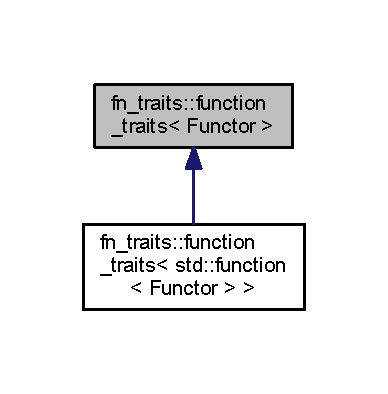
\includegraphics[width=186pt]{df/da7/structfn__traits_1_1function__traits__inherit__graph}
\end{center}
\end{figure}


\subsection{Detailed Description}
\subsubsection*{template$<$typename Functor$>$\\*
struct fn\+\_\+traits\+::function\+\_\+traits$<$ Functor $>$}



Definition at line 16 of file function\+\_\+traits.\+hpp.



The documentation for this struct was generated from the following file\+:\begin{DoxyCompactItemize}
\item 
include/\hyperlink{function__traits_8hpp}{function\+\_\+traits.\+hpp}\end{DoxyCompactItemize}

\hypertarget{structfn__traits_1_1function__traits_3_01const_01_t_01_6_01_4}{}\section{fn\+\_\+traits\+:\+:function\+\_\+traits$<$ const T \& $>$ Struct Template Reference}
\label{structfn__traits_1_1function__traits_3_01const_01_t_01_6_01_4}\index{fn\+\_\+traits\+::function\+\_\+traits$<$ const T \& $>$@{fn\+\_\+traits\+::function\+\_\+traits$<$ const T \& $>$}}


{\ttfamily \#include $<$function\+\_\+traits.\+hpp$>$}



Inheritance diagram for fn\+\_\+traits\+:\+:function\+\_\+traits$<$ const T \& $>$\+:\nopagebreak
\begin{figure}[H]
\begin{center}
\leavevmode
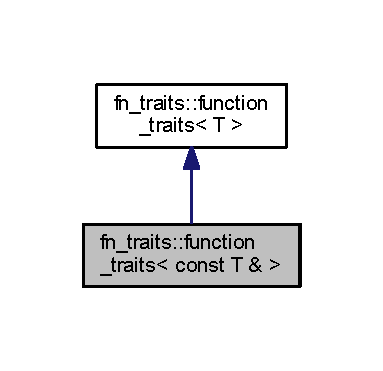
\includegraphics[width=184pt]{d2/dcd/structfn__traits_1_1function__traits_3_01const_01_t_01_6_01_4__inherit__graph}
\end{center}
\end{figure}


Collaboration diagram for fn\+\_\+traits\+:\+:function\+\_\+traits$<$ const T \& $>$\+:\nopagebreak
\begin{figure}[H]
\begin{center}
\leavevmode
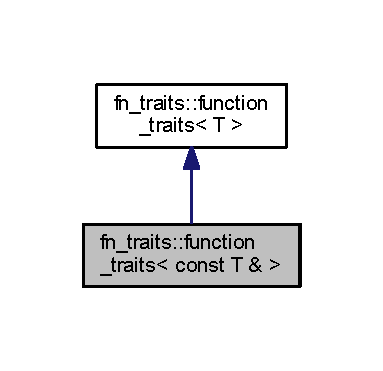
\includegraphics[width=184pt]{db/d00/structfn__traits_1_1function__traits_3_01const_01_t_01_6_01_4__coll__graph}
\end{center}
\end{figure}


\subsection{Detailed Description}
\subsubsection*{template$<$typename T$>$\\*
struct fn\+\_\+traits\+::function\+\_\+traits$<$ const T \& $>$}



Definition at line 118 of file function\+\_\+traits.\+hpp.



The documentation for this struct was generated from the following file\+:\begin{DoxyCompactItemize}
\item 
include/\hyperlink{function__traits_8hpp}{function\+\_\+traits.\+hpp}\end{DoxyCompactItemize}

\hypertarget{structfn__traits_1_1function__traits_3_01const_01_t_01_6_6_01_4}{}\section{fn\+\_\+traits\+:\+:function\+\_\+traits$<$ const T \&\& $>$ Struct Template Reference}
\label{structfn__traits_1_1function__traits_3_01const_01_t_01_6_6_01_4}\index{fn\+\_\+traits\+::function\+\_\+traits$<$ const T \&\& $>$@{fn\+\_\+traits\+::function\+\_\+traits$<$ const T \&\& $>$}}


{\ttfamily \#include $<$function\+\_\+traits.\+hpp$>$}



Inheritance diagram for fn\+\_\+traits\+:\+:function\+\_\+traits$<$ const T \&\& $>$\+:\nopagebreak
\begin{figure}[H]
\begin{center}
\leavevmode
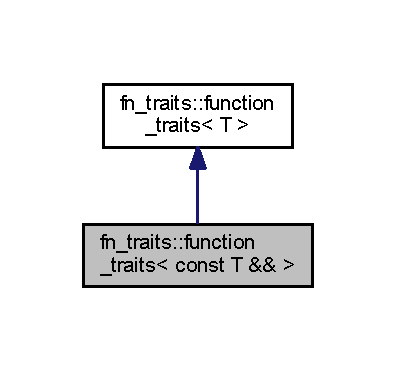
\includegraphics[width=190pt]{d9/daa/structfn__traits_1_1function__traits_3_01const_01_t_01_6_6_01_4__inherit__graph}
\end{center}
\end{figure}


Collaboration diagram for fn\+\_\+traits\+:\+:function\+\_\+traits$<$ const T \&\& $>$\+:\nopagebreak
\begin{figure}[H]
\begin{center}
\leavevmode
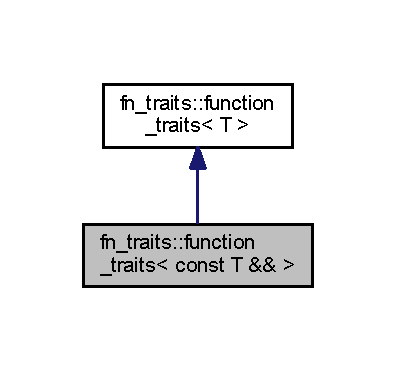
\includegraphics[width=190pt]{de/db9/structfn__traits_1_1function__traits_3_01const_01_t_01_6_6_01_4__coll__graph}
\end{center}
\end{figure}


\subsection{Detailed Description}
\subsubsection*{template$<$typename T$>$\\*
struct fn\+\_\+traits\+::function\+\_\+traits$<$ const T \&\& $>$}



Definition at line 134 of file function\+\_\+traits.\+hpp.



The documentation for this struct was generated from the following file\+:\begin{DoxyCompactItemize}
\item 
include/\hyperlink{function__traits_8hpp}{function\+\_\+traits.\+hpp}\end{DoxyCompactItemize}

\hypertarget{structfn__traits_1_1function__traits_3_01const_01volatile_01_t_01_6_01_4}{}\section{fn\+\_\+traits\+:\+:function\+\_\+traits$<$ const volatile T \& $>$ Struct Template Reference}
\label{structfn__traits_1_1function__traits_3_01const_01volatile_01_t_01_6_01_4}\index{fn\+\_\+traits\+::function\+\_\+traits$<$ const volatile T \& $>$@{fn\+\_\+traits\+::function\+\_\+traits$<$ const volatile T \& $>$}}


{\ttfamily \#include $<$function\+\_\+traits.\+hpp$>$}



Inheritance diagram for fn\+\_\+traits\+:\+:function\+\_\+traits$<$ const volatile T \& $>$\+:\nopagebreak
\begin{figure}[H]
\begin{center}
\leavevmode
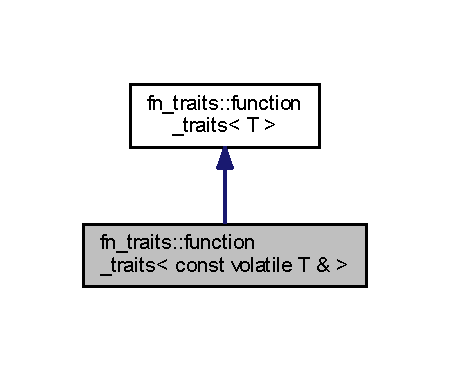
\includegraphics[width=216pt]{de/dbb/structfn__traits_1_1function__traits_3_01const_01volatile_01_t_01_6_01_4__inherit__graph}
\end{center}
\end{figure}


Collaboration diagram for fn\+\_\+traits\+:\+:function\+\_\+traits$<$ const volatile T \& $>$\+:\nopagebreak
\begin{figure}[H]
\begin{center}
\leavevmode
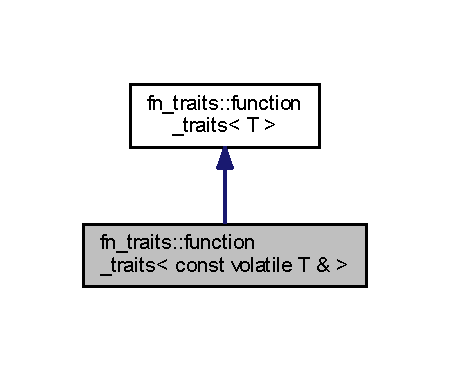
\includegraphics[width=216pt]{d6/df7/structfn__traits_1_1function__traits_3_01const_01volatile_01_t_01_6_01_4__coll__graph}
\end{center}
\end{figure}


\subsection{Detailed Description}
\subsubsection*{template$<$typename T$>$\\*
struct fn\+\_\+traits\+::function\+\_\+traits$<$ const volatile T \& $>$}



Definition at line 126 of file function\+\_\+traits.\+hpp.



The documentation for this struct was generated from the following file\+:\begin{DoxyCompactItemize}
\item 
include/\hyperlink{function__traits_8hpp}{function\+\_\+traits.\+hpp}\end{DoxyCompactItemize}

\hypertarget{structfn__traits_1_1function__traits_3_01const_01volatile_01_t_01_6_6_01_4}{}\section{fn\+\_\+traits\+:\+:function\+\_\+traits$<$ const volatile T \&\& $>$ Struct Template Reference}
\label{structfn__traits_1_1function__traits_3_01const_01volatile_01_t_01_6_6_01_4}\index{fn\+\_\+traits\+::function\+\_\+traits$<$ const volatile T \&\& $>$@{fn\+\_\+traits\+::function\+\_\+traits$<$ const volatile T \&\& $>$}}


{\ttfamily \#include $<$function\+\_\+traits.\+hpp$>$}



Inheritance diagram for fn\+\_\+traits\+:\+:function\+\_\+traits$<$ const volatile T \&\& $>$\+:\nopagebreak
\begin{figure}[H]
\begin{center}
\leavevmode
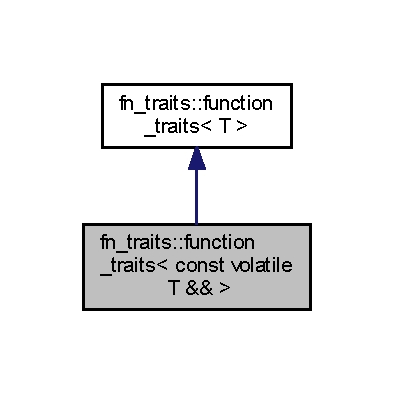
\includegraphics[width=189pt]{d9/dea/structfn__traits_1_1function__traits_3_01const_01volatile_01_t_01_6_6_01_4__inherit__graph}
\end{center}
\end{figure}


Collaboration diagram for fn\+\_\+traits\+:\+:function\+\_\+traits$<$ const volatile T \&\& $>$\+:\nopagebreak
\begin{figure}[H]
\begin{center}
\leavevmode
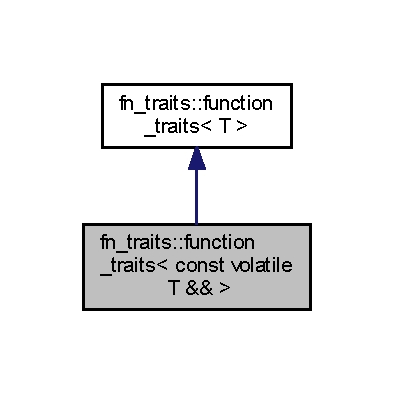
\includegraphics[width=189pt]{d3/de4/structfn__traits_1_1function__traits_3_01const_01volatile_01_t_01_6_6_01_4__coll__graph}
\end{center}
\end{figure}


\subsection{Detailed Description}
\subsubsection*{template$<$typename T$>$\\*
struct fn\+\_\+traits\+::function\+\_\+traits$<$ const volatile T \&\& $>$}



Definition at line 142 of file function\+\_\+traits.\+hpp.



The documentation for this struct was generated from the following file\+:\begin{DoxyCompactItemize}
\item 
include/\hyperlink{function__traits_8hpp}{function\+\_\+traits.\+hpp}\end{DoxyCompactItemize}

\hypertarget{structfn__traits_1_1function__traits_3_01_r_07_5_08_07_args_8_8_8_08_4}{}\section{fn\+\_\+traits\+:\+:function\+\_\+traits$<$ R($\ast$)(Args...)$>$ Struct Template Reference}
\label{structfn__traits_1_1function__traits_3_01_r_07_5_08_07_args_8_8_8_08_4}\index{fn\+\_\+traits\+::function\+\_\+traits$<$ R($\ast$)(\+Args...)$>$@{fn\+\_\+traits\+::function\+\_\+traits$<$ R($\ast$)(\+Args...)$>$}}


{\ttfamily \#include $<$function\+\_\+traits.\+hpp$>$}



Inheritance diagram for fn\+\_\+traits\+:\+:function\+\_\+traits$<$ R($\ast$)(Args...)$>$\+:\nopagebreak
\begin{figure}[H]
\begin{center}
\leavevmode
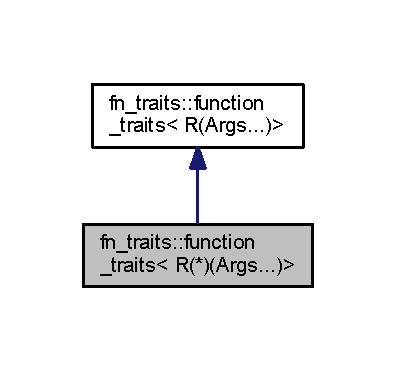
\includegraphics[width=190pt]{de/df9/structfn__traits_1_1function__traits_3_01_r_07_5_08_07_args_8_8_8_08_4__inherit__graph}
\end{center}
\end{figure}


Collaboration diagram for fn\+\_\+traits\+:\+:function\+\_\+traits$<$ R($\ast$)(Args...)$>$\+:\nopagebreak
\begin{figure}[H]
\begin{center}
\leavevmode
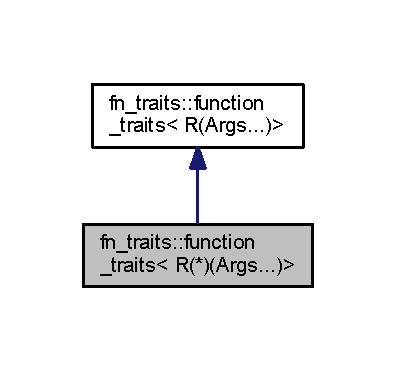
\includegraphics[width=190pt]{df/db5/structfn__traits_1_1function__traits_3_01_r_07_5_08_07_args_8_8_8_08_4__coll__graph}
\end{center}
\end{figure}
\subsection*{Public Types}
\begin{DoxyCompactItemize}
\item 
enum \{ \hyperlink{structfn__traits_1_1function__traits_3_01_r_07_args_8_8_8_08_4_aafde9521d9646c97b984646d8273dd3ba2f612b5524050ab8d6ab3d54d52dbbb0}{arity} = sizeof...( Args )
 \}
\item 
typedef R \hyperlink{structfn__traits_1_1function__traits_3_01_r_07_args_8_8_8_08_4_a1b509243ed1b4707465625de10e6c6bb}{result\+\_\+type}
\item 
typedef \hyperlink{structfn__traits_1_1function__traits_3_01_r_07_args_8_8_8_08_4_a1b509243ed1b4707465625de10e6c6bb}{result\+\_\+type} \hyperlink{structfn__traits_1_1function__traits_3_01_r_07_args_8_8_8_08_4_adf6a35a9b703dfb4778e59f132e00a9b}{return\+\_\+type}
\item 
typedef \hyperlink{structfn__traits_1_1function__traits_3_01_r_07_args_8_8_8_08_4_a1b509243ed1b4707465625de10e6c6bb}{result\+\_\+type} \hyperlink{structfn__traits_1_1function__traits_3_01_r_07_args_8_8_8_08_4_a85e5883a1c8050fe442c1072386b2d11}{function\+\_\+type}(Args...)
\item 
typedef std\+::tuple$<$ Args... $>$ \hyperlink{structfn__traits_1_1function__traits_3_01_r_07_args_8_8_8_08_4_a9b60ae8c79e52addf352e4ae7c8077b4}{tuple\+\_\+type}
\end{DoxyCompactItemize}


\subsection{Detailed Description}
\subsubsection*{template$<$typename R, typename... Args$>$\\*
struct fn\+\_\+traits\+::function\+\_\+traits$<$ R($\ast$)(\+Args...)$>$}



Definition at line 41 of file function\+\_\+traits.\+hpp.



\subsection{Member Typedef Documentation}
\index{fn\+\_\+traits\+::function\+\_\+traits$<$ R($\ast$)(\+Args...)$>$@{fn\+\_\+traits\+::function\+\_\+traits$<$ R($\ast$)(\+Args...)$>$}!function\+\_\+type@{function\+\_\+type}}
\index{function\+\_\+type@{function\+\_\+type}!fn\+\_\+traits\+::function\+\_\+traits$<$ R($\ast$)(\+Args...)$>$@{fn\+\_\+traits\+::function\+\_\+traits$<$ R($\ast$)(\+Args...)$>$}}
\subsubsection[{\texorpdfstring{function\+\_\+type}{function_type}}]{\setlength{\rightskip}{0pt plus 5cm}template$<$typename R , typename... Args$>$ typedef {\bf result\+\_\+type} {\bf fn\+\_\+traits\+::function\+\_\+traits}$<$ R(Args...)$>$\+::function\+\_\+type(Args...)\hspace{0.3cm}{\ttfamily [inherited]}}\hypertarget{structfn__traits_1_1function__traits_3_01_r_07_args_8_8_8_08_4_a85e5883a1c8050fe442c1072386b2d11}{}\label{structfn__traits_1_1function__traits_3_01_r_07_args_8_8_8_08_4_a85e5883a1c8050fe442c1072386b2d11}


Definition at line 26 of file function\+\_\+traits.\+hpp.

\index{fn\+\_\+traits\+::function\+\_\+traits$<$ R($\ast$)(\+Args...)$>$@{fn\+\_\+traits\+::function\+\_\+traits$<$ R($\ast$)(\+Args...)$>$}!result\+\_\+type@{result\+\_\+type}}
\index{result\+\_\+type@{result\+\_\+type}!fn\+\_\+traits\+::function\+\_\+traits$<$ R($\ast$)(\+Args...)$>$@{fn\+\_\+traits\+::function\+\_\+traits$<$ R($\ast$)(\+Args...)$>$}}
\subsubsection[{\texorpdfstring{result\+\_\+type}{result_type}}]{\setlength{\rightskip}{0pt plus 5cm}template$<$typename R , typename... Args$>$ typedef R {\bf fn\+\_\+traits\+::function\+\_\+traits}$<$ R(Args...)$>$\+::{\bf result\+\_\+type}\hspace{0.3cm}{\ttfamily [inherited]}}\hypertarget{structfn__traits_1_1function__traits_3_01_r_07_args_8_8_8_08_4_a1b509243ed1b4707465625de10e6c6bb}{}\label{structfn__traits_1_1function__traits_3_01_r_07_args_8_8_8_08_4_a1b509243ed1b4707465625de10e6c6bb}


Definition at line 22 of file function\+\_\+traits.\+hpp.

\index{fn\+\_\+traits\+::function\+\_\+traits$<$ R($\ast$)(\+Args...)$>$@{fn\+\_\+traits\+::function\+\_\+traits$<$ R($\ast$)(\+Args...)$>$}!return\+\_\+type@{return\+\_\+type}}
\index{return\+\_\+type@{return\+\_\+type}!fn\+\_\+traits\+::function\+\_\+traits$<$ R($\ast$)(\+Args...)$>$@{fn\+\_\+traits\+::function\+\_\+traits$<$ R($\ast$)(\+Args...)$>$}}
\subsubsection[{\texorpdfstring{return\+\_\+type}{return_type}}]{\setlength{\rightskip}{0pt plus 5cm}template$<$typename R , typename... Args$>$ typedef {\bf result\+\_\+type} {\bf fn\+\_\+traits\+::function\+\_\+traits}$<$ R(Args...)$>$\+::{\bf return\+\_\+type}\hspace{0.3cm}{\ttfamily [inherited]}}\hypertarget{structfn__traits_1_1function__traits_3_01_r_07_args_8_8_8_08_4_adf6a35a9b703dfb4778e59f132e00a9b}{}\label{structfn__traits_1_1function__traits_3_01_r_07_args_8_8_8_08_4_adf6a35a9b703dfb4778e59f132e00a9b}


Definition at line 24 of file function\+\_\+traits.\+hpp.

\index{fn\+\_\+traits\+::function\+\_\+traits$<$ R($\ast$)(\+Args...)$>$@{fn\+\_\+traits\+::function\+\_\+traits$<$ R($\ast$)(\+Args...)$>$}!tuple\+\_\+type@{tuple\+\_\+type}}
\index{tuple\+\_\+type@{tuple\+\_\+type}!fn\+\_\+traits\+::function\+\_\+traits$<$ R($\ast$)(\+Args...)$>$@{fn\+\_\+traits\+::function\+\_\+traits$<$ R($\ast$)(\+Args...)$>$}}
\subsubsection[{\texorpdfstring{tuple\+\_\+type}{tuple_type}}]{\setlength{\rightskip}{0pt plus 5cm}template$<$typename R , typename... Args$>$ typedef std\+::tuple$<$Args...$>$ {\bf fn\+\_\+traits\+::function\+\_\+traits}$<$ R(Args...)$>$\+::{\bf tuple\+\_\+type}\hspace{0.3cm}{\ttfamily [inherited]}}\hypertarget{structfn__traits_1_1function__traits_3_01_r_07_args_8_8_8_08_4_a9b60ae8c79e52addf352e4ae7c8077b4}{}\label{structfn__traits_1_1function__traits_3_01_r_07_args_8_8_8_08_4_a9b60ae8c79e52addf352e4ae7c8077b4}


Definition at line 32 of file function\+\_\+traits.\+hpp.



\subsection{Member Enumeration Documentation}
\subsubsection[{\texorpdfstring{anonymous enum}{anonymous enum}}]{\setlength{\rightskip}{0pt plus 5cm}template$<$typename R , typename... Args$>$ anonymous enum\hspace{0.3cm}{\ttfamily [inherited]}}\hypertarget{structfn__traits_1_1function__traits_3_01_r_07_args_8_8_8_08_4_aafde9521d9646c97b984646d8273dd3b}{}\label{structfn__traits_1_1function__traits_3_01_r_07_args_8_8_8_08_4_aafde9521d9646c97b984646d8273dd3b}
\begin{Desc}
\item[Enumerator]\par
\begin{description}
\index{arity@{arity}!fn\+\_\+traits\+::function\+\_\+traits$<$ R($\ast$)(\+Args...)$>$@{fn\+\_\+traits\+::function\+\_\+traits$<$ R($\ast$)(\+Args...)$>$}}\index{fn\+\_\+traits\+::function\+\_\+traits$<$ R($\ast$)(\+Args...)$>$@{fn\+\_\+traits\+::function\+\_\+traits$<$ R($\ast$)(\+Args...)$>$}!arity@{arity}}\item[{\em 
arity\hypertarget{structfn__traits_1_1function__traits_3_01_r_07_args_8_8_8_08_4_aafde9521d9646c97b984646d8273dd3ba2f612b5524050ab8d6ab3d54d52dbbb0}{}\label{structfn__traits_1_1function__traits_3_01_r_07_args_8_8_8_08_4_aafde9521d9646c97b984646d8273dd3ba2f612b5524050ab8d6ab3d54d52dbbb0}
}]\end{description}
\end{Desc}


Definition at line 28 of file function\+\_\+traits.\+hpp.


\begin{DoxyCode}
28              \{
29             \hyperlink{structfn__traits_1_1function__traits_3_01_r_07_args_8_8_8_08_4_aafde9521d9646c97b984646d8273dd3ba2f612b5524050ab8d6ab3d54d52dbbb0}{arity} = \textcolor{keyword}{sizeof}...( Args )
30         \};
\end{DoxyCode}


The documentation for this struct was generated from the following file\+:\begin{DoxyCompactItemize}
\item 
include/\hyperlink{function__traits_8hpp}{function\+\_\+traits.\+hpp}\end{DoxyCompactItemize}

\hypertarget{structfn__traits_1_1function__traits_3_01_r_07_args_8_8_8_08_4}{}\section{fn\+\_\+traits\+:\+:function\+\_\+traits$<$ R(Args...)$>$ Struct Template Reference}
\label{structfn__traits_1_1function__traits_3_01_r_07_args_8_8_8_08_4}\index{fn\+\_\+traits\+::function\+\_\+traits$<$ R(\+Args...)$>$@{fn\+\_\+traits\+::function\+\_\+traits$<$ R(\+Args...)$>$}}


{\ttfamily \#include $<$function\+\_\+traits.\+hpp$>$}



Inheritance diagram for fn\+\_\+traits\+:\+:function\+\_\+traits$<$ R(Args...)$>$\+:\nopagebreak
\begin{figure}[H]
\begin{center}
\leavevmode
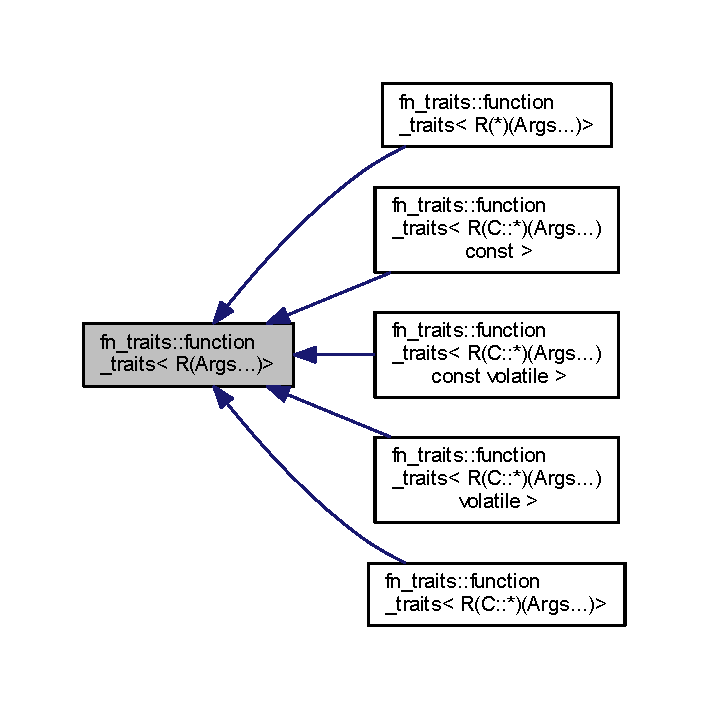
\includegraphics[width=340pt]{d7/d7c/structfn__traits_1_1function__traits_3_01_r_07_args_8_8_8_08_4__inherit__graph}
\end{center}
\end{figure}
\subsection*{Classes}
\begin{DoxyCompactItemize}
\item 
struct \hyperlink{structfn__traits_1_1function__traits_3_01_r_07_args_8_8_8_08_4_d9/d01/structfn__traits_1_1function__traits_3_01_r_07_args_8_8_8_08_4_1_1arg}{arg}
\end{DoxyCompactItemize}
\subsection*{Public Types}
\begin{DoxyCompactItemize}
\item 
enum \{ \hyperlink{structfn__traits_1_1function__traits_3_01_r_07_args_8_8_8_08_4_aafde9521d9646c97b984646d8273dd3ba2f612b5524050ab8d6ab3d54d52dbbb0}{arity} = sizeof...( Args )
 \}
\item 
typedef R \hyperlink{structfn__traits_1_1function__traits_3_01_r_07_args_8_8_8_08_4_a1b509243ed1b4707465625de10e6c6bb}{result\+\_\+type}
\item 
typedef \hyperlink{structfn__traits_1_1function__traits_3_01_r_07_args_8_8_8_08_4_a1b509243ed1b4707465625de10e6c6bb}{result\+\_\+type} \hyperlink{structfn__traits_1_1function__traits_3_01_r_07_args_8_8_8_08_4_adf6a35a9b703dfb4778e59f132e00a9b}{return\+\_\+type}
\item 
typedef \hyperlink{structfn__traits_1_1function__traits_3_01_r_07_args_8_8_8_08_4_a1b509243ed1b4707465625de10e6c6bb}{result\+\_\+type} \hyperlink{structfn__traits_1_1function__traits_3_01_r_07_args_8_8_8_08_4_a85e5883a1c8050fe442c1072386b2d11}{function\+\_\+type}(Args...)
\item 
typedef std\+::tuple$<$ Args... $>$ \hyperlink{structfn__traits_1_1function__traits_3_01_r_07_args_8_8_8_08_4_a9b60ae8c79e52addf352e4ae7c8077b4}{tuple\+\_\+type}
\end{DoxyCompactItemize}


\subsection{Detailed Description}
\subsubsection*{template$<$typename R, typename... Args$>$\\*
struct fn\+\_\+traits\+::function\+\_\+traits$<$ R(\+Args...)$>$}



Definition at line 21 of file function\+\_\+traits.\+hpp.



\subsection{Class Documentation}
\index{fn\+\_\+traits\+::function\+\_\+traits$<$ R(\+Args...)$>$\+::arg@{fn\+\_\+traits\+::function\+\_\+traits$<$ R(\+Args...)$>$\+::arg}}\label{structfn__traits_1_1function__traits_3_01_r_07_args_8_8_8_08_4_1_1arg}
\hypertarget{structfn__traits_1_1function__traits_3_01_r_07_args_8_8_8_08_4_structfn__traits_1_1function__traits_3_01_r_07_args_8_8_8_08_4_1_1arg}{}
\subsubsection{struct fn\+\_\+traits\+:\+:function\+\_\+traits$<$ R(Args...)$>$\+:\+:arg}
\subsubsection*{template$<$typename R, typename... Args$>$\\*
template$<$size\+\_\+t i$>$\\*
struct fn\+\_\+traits\+::function\+\_\+traits$<$ R(\+Args...)$>$\+::arg$<$ i $>$}



Definition at line 35 of file function\+\_\+traits.\+hpp.

\begin{DoxyFields}{Class Members}
typedef tuple\+\_\+element$<$ i, \\*
\hyperlink{structfn__traits_1_1function__traits_3_01_r_07_args_8_8_8_08_4_a9b60ae8c79e52addf352e4ae7c8077b4}{tuple\+\_\+type} $>$\+::\hyperlink{structfn__traits_1_1function__traits_3_01_r_07_args_8_8_8_08_4_ac0fde1bea9167cdc37a22b37bea78eb3}{type}\hypertarget{structfn__traits_1_1function__traits_3_01_r_07_args_8_8_8_08_4_ac0fde1bea9167cdc37a22b37bea78eb3}{}\label{structfn__traits_1_1function__traits_3_01_r_07_args_8_8_8_08_4_ac0fde1bea9167cdc37a22b37bea78eb3}
&
type&
\\
\hline

\end{DoxyFields}


\subsection{Member Typedef Documentation}
\index{fn\+\_\+traits\+::function\+\_\+traits$<$ R(\+Args...)$>$@{fn\+\_\+traits\+::function\+\_\+traits$<$ R(\+Args...)$>$}!function\+\_\+type@{function\+\_\+type}}
\index{function\+\_\+type@{function\+\_\+type}!fn\+\_\+traits\+::function\+\_\+traits$<$ R(\+Args...)$>$@{fn\+\_\+traits\+::function\+\_\+traits$<$ R(\+Args...)$>$}}
\subsubsection[{\texorpdfstring{function\+\_\+type}{function_type}}]{\setlength{\rightskip}{0pt plus 5cm}template$<$typename R , typename... Args$>$ typedef {\bf result\+\_\+type} {\bf fn\+\_\+traits\+::function\+\_\+traits}$<$ R(Args...)$>$\+::function\+\_\+type(Args...)}\hypertarget{structfn__traits_1_1function__traits_3_01_r_07_args_8_8_8_08_4_a85e5883a1c8050fe442c1072386b2d11}{}\label{structfn__traits_1_1function__traits_3_01_r_07_args_8_8_8_08_4_a85e5883a1c8050fe442c1072386b2d11}


Definition at line 26 of file function\+\_\+traits.\+hpp.

\index{fn\+\_\+traits\+::function\+\_\+traits$<$ R(\+Args...)$>$@{fn\+\_\+traits\+::function\+\_\+traits$<$ R(\+Args...)$>$}!result\+\_\+type@{result\+\_\+type}}
\index{result\+\_\+type@{result\+\_\+type}!fn\+\_\+traits\+::function\+\_\+traits$<$ R(\+Args...)$>$@{fn\+\_\+traits\+::function\+\_\+traits$<$ R(\+Args...)$>$}}
\subsubsection[{\texorpdfstring{result\+\_\+type}{result_type}}]{\setlength{\rightskip}{0pt plus 5cm}template$<$typename R , typename... Args$>$ typedef R {\bf fn\+\_\+traits\+::function\+\_\+traits}$<$ R(Args...)$>$\+::{\bf result\+\_\+type}}\hypertarget{structfn__traits_1_1function__traits_3_01_r_07_args_8_8_8_08_4_a1b509243ed1b4707465625de10e6c6bb}{}\label{structfn__traits_1_1function__traits_3_01_r_07_args_8_8_8_08_4_a1b509243ed1b4707465625de10e6c6bb}


Definition at line 22 of file function\+\_\+traits.\+hpp.

\index{fn\+\_\+traits\+::function\+\_\+traits$<$ R(\+Args...)$>$@{fn\+\_\+traits\+::function\+\_\+traits$<$ R(\+Args...)$>$}!return\+\_\+type@{return\+\_\+type}}
\index{return\+\_\+type@{return\+\_\+type}!fn\+\_\+traits\+::function\+\_\+traits$<$ R(\+Args...)$>$@{fn\+\_\+traits\+::function\+\_\+traits$<$ R(\+Args...)$>$}}
\subsubsection[{\texorpdfstring{return\+\_\+type}{return_type}}]{\setlength{\rightskip}{0pt plus 5cm}template$<$typename R , typename... Args$>$ typedef {\bf result\+\_\+type} {\bf fn\+\_\+traits\+::function\+\_\+traits}$<$ R(Args...)$>$\+::{\bf return\+\_\+type}}\hypertarget{structfn__traits_1_1function__traits_3_01_r_07_args_8_8_8_08_4_adf6a35a9b703dfb4778e59f132e00a9b}{}\label{structfn__traits_1_1function__traits_3_01_r_07_args_8_8_8_08_4_adf6a35a9b703dfb4778e59f132e00a9b}


Definition at line 24 of file function\+\_\+traits.\+hpp.

\index{fn\+\_\+traits\+::function\+\_\+traits$<$ R(\+Args...)$>$@{fn\+\_\+traits\+::function\+\_\+traits$<$ R(\+Args...)$>$}!tuple\+\_\+type@{tuple\+\_\+type}}
\index{tuple\+\_\+type@{tuple\+\_\+type}!fn\+\_\+traits\+::function\+\_\+traits$<$ R(\+Args...)$>$@{fn\+\_\+traits\+::function\+\_\+traits$<$ R(\+Args...)$>$}}
\subsubsection[{\texorpdfstring{tuple\+\_\+type}{tuple_type}}]{\setlength{\rightskip}{0pt plus 5cm}template$<$typename R , typename... Args$>$ typedef std\+::tuple$<$Args...$>$ {\bf fn\+\_\+traits\+::function\+\_\+traits}$<$ R(Args...)$>$\+::{\bf tuple\+\_\+type}}\hypertarget{structfn__traits_1_1function__traits_3_01_r_07_args_8_8_8_08_4_a9b60ae8c79e52addf352e4ae7c8077b4}{}\label{structfn__traits_1_1function__traits_3_01_r_07_args_8_8_8_08_4_a9b60ae8c79e52addf352e4ae7c8077b4}


Definition at line 32 of file function\+\_\+traits.\+hpp.



\subsection{Member Enumeration Documentation}
\subsubsection[{\texorpdfstring{anonymous enum}{anonymous enum}}]{\setlength{\rightskip}{0pt plus 5cm}template$<$typename R , typename... Args$>$ anonymous enum}\hypertarget{structfn__traits_1_1function__traits_3_01_r_07_args_8_8_8_08_4_aafde9521d9646c97b984646d8273dd3b}{}\label{structfn__traits_1_1function__traits_3_01_r_07_args_8_8_8_08_4_aafde9521d9646c97b984646d8273dd3b}
\begin{Desc}
\item[Enumerator]\par
\begin{description}
\index{arity@{arity}!fn\+\_\+traits\+::function\+\_\+traits$<$ R(\+Args...)$>$@{fn\+\_\+traits\+::function\+\_\+traits$<$ R(\+Args...)$>$}}\index{fn\+\_\+traits\+::function\+\_\+traits$<$ R(\+Args...)$>$@{fn\+\_\+traits\+::function\+\_\+traits$<$ R(\+Args...)$>$}!arity@{arity}}\item[{\em 
arity\hypertarget{structfn__traits_1_1function__traits_3_01_r_07_args_8_8_8_08_4_aafde9521d9646c97b984646d8273dd3ba2f612b5524050ab8d6ab3d54d52dbbb0}{}\label{structfn__traits_1_1function__traits_3_01_r_07_args_8_8_8_08_4_aafde9521d9646c97b984646d8273dd3ba2f612b5524050ab8d6ab3d54d52dbbb0}
}]\end{description}
\end{Desc}


Definition at line 28 of file function\+\_\+traits.\+hpp.


\begin{DoxyCode}
28              \{
29             \hyperlink{structfn__traits_1_1function__traits_3_01_r_07_args_8_8_8_08_4_aafde9521d9646c97b984646d8273dd3ba2f612b5524050ab8d6ab3d54d52dbbb0}{arity} = \textcolor{keyword}{sizeof}...( Args )
30         \};
\end{DoxyCode}


The documentation for this struct was generated from the following file\+:\begin{DoxyCompactItemize}
\item 
include/\hyperlink{function__traits_8hpp}{function\+\_\+traits.\+hpp}\end{DoxyCompactItemize}

\hypertarget{structfn__traits_1_1function__traits_3_01_r_07_c_1_1_5_08_07_args_8_8_8_08_01const_01_01_4}{}\section{fn\+\_\+traits\+:\+:function\+\_\+traits$<$ R(C\+:\+:$\ast$)(Args...) const $>$ Struct Template Reference}
\label{structfn__traits_1_1function__traits_3_01_r_07_c_1_1_5_08_07_args_8_8_8_08_01const_01_01_4}\index{fn\+\_\+traits\+::function\+\_\+traits$<$ R(\+C\+::$\ast$)(\+Args...) const  $>$@{fn\+\_\+traits\+::function\+\_\+traits$<$ R(\+C\+::$\ast$)(\+Args...) const  $>$}}


{\ttfamily \#include $<$function\+\_\+traits.\+hpp$>$}



Inheritance diagram for fn\+\_\+traits\+:\+:function\+\_\+traits$<$ R(C\+:\+:$\ast$)(Args...) const $>$\+:\nopagebreak
\begin{figure}[H]
\begin{center}
\leavevmode
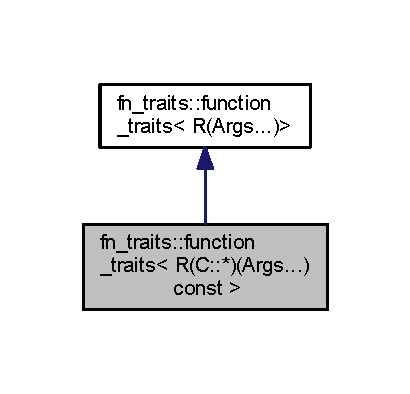
\includegraphics[width=197pt]{d2/dda/structfn__traits_1_1function__traits_3_01_r_07_c_1_1_5_08_07_args_8_8_8_08_01const_01_01_4__inherit__graph}
\end{center}
\end{figure}


Collaboration diagram for fn\+\_\+traits\+:\+:function\+\_\+traits$<$ R(C\+:\+:$\ast$)(Args...) const $>$\+:\nopagebreak
\begin{figure}[H]
\begin{center}
\leavevmode
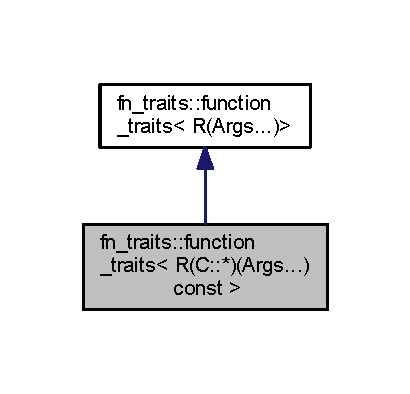
\includegraphics[width=197pt]{d7/d7f/structfn__traits_1_1function__traits_3_01_r_07_c_1_1_5_08_07_args_8_8_8_08_01const_01_01_4__coll__graph}
\end{center}
\end{figure}
\subsection*{Public Types}
\begin{DoxyCompactItemize}
\item 
typedef const C \& \hyperlink{structfn__traits_1_1function__traits_3_01_r_07_c_1_1_5_08_07_args_8_8_8_08_01const_01_01_4_af861070a9fa7ecbcc812135e16232e9a}{owner\+\_\+type}
\item 
enum \{ \hyperlink{structfn__traits_1_1function__traits_3_01_r_07_args_8_8_8_08_4_aafde9521d9646c97b984646d8273dd3ba2f612b5524050ab8d6ab3d54d52dbbb0}{arity} = sizeof...( Args )
 \}
\item 
typedef R \hyperlink{structfn__traits_1_1function__traits_3_01_r_07_args_8_8_8_08_4_a1b509243ed1b4707465625de10e6c6bb}{result\+\_\+type}
\item 
typedef \hyperlink{structfn__traits_1_1function__traits_3_01_r_07_args_8_8_8_08_4_a1b509243ed1b4707465625de10e6c6bb}{result\+\_\+type} \hyperlink{structfn__traits_1_1function__traits_3_01_r_07_args_8_8_8_08_4_adf6a35a9b703dfb4778e59f132e00a9b}{return\+\_\+type}
\item 
typedef \hyperlink{structfn__traits_1_1function__traits_3_01_r_07_args_8_8_8_08_4_a1b509243ed1b4707465625de10e6c6bb}{result\+\_\+type} \hyperlink{structfn__traits_1_1function__traits_3_01_r_07_args_8_8_8_08_4_a85e5883a1c8050fe442c1072386b2d11}{function\+\_\+type}(Args...)
\item 
typedef std\+::tuple$<$ Args... $>$ \hyperlink{structfn__traits_1_1function__traits_3_01_r_07_args_8_8_8_08_4_a9b60ae8c79e52addf352e4ae7c8077b4}{tuple\+\_\+type}
\end{DoxyCompactItemize}


\subsection{Detailed Description}
\subsubsection*{template$<$typename C, typename R, typename... Args$>$\\*
struct fn\+\_\+traits\+::function\+\_\+traits$<$ R(\+C\+::$\ast$)(\+Args...) const  $>$}



Definition at line 52 of file function\+\_\+traits.\+hpp.



\subsection{Member Typedef Documentation}
\index{fn\+\_\+traits\+::function\+\_\+traits$<$ R(\+C\+::$\ast$)(\+Args...) const  $>$@{fn\+\_\+traits\+::function\+\_\+traits$<$ R(\+C\+::$\ast$)(\+Args...) const  $>$}!function\+\_\+type@{function\+\_\+type}}
\index{function\+\_\+type@{function\+\_\+type}!fn\+\_\+traits\+::function\+\_\+traits$<$ R(\+C\+::$\ast$)(\+Args...) const  $>$@{fn\+\_\+traits\+::function\+\_\+traits$<$ R(\+C\+::$\ast$)(\+Args...) const  $>$}}
\subsubsection[{\texorpdfstring{function\+\_\+type}{function_type}}]{\setlength{\rightskip}{0pt plus 5cm}template$<$typename R , typename... Args$>$ typedef {\bf result\+\_\+type} {\bf fn\+\_\+traits\+::function\+\_\+traits}$<$ R(Args...)$>$\+::function\+\_\+type(Args...)\hspace{0.3cm}{\ttfamily [inherited]}}\hypertarget{structfn__traits_1_1function__traits_3_01_r_07_args_8_8_8_08_4_a85e5883a1c8050fe442c1072386b2d11}{}\label{structfn__traits_1_1function__traits_3_01_r_07_args_8_8_8_08_4_a85e5883a1c8050fe442c1072386b2d11}


Definition at line 26 of file function\+\_\+traits.\+hpp.

\index{fn\+\_\+traits\+::function\+\_\+traits$<$ R(\+C\+::$\ast$)(\+Args...) const  $>$@{fn\+\_\+traits\+::function\+\_\+traits$<$ R(\+C\+::$\ast$)(\+Args...) const  $>$}!owner\+\_\+type@{owner\+\_\+type}}
\index{owner\+\_\+type@{owner\+\_\+type}!fn\+\_\+traits\+::function\+\_\+traits$<$ R(\+C\+::$\ast$)(\+Args...) const  $>$@{fn\+\_\+traits\+::function\+\_\+traits$<$ R(\+C\+::$\ast$)(\+Args...) const  $>$}}
\subsubsection[{\texorpdfstring{owner\+\_\+type}{owner_type}}]{\setlength{\rightskip}{0pt plus 5cm}template$<$typename C , typename R , typename... Args$>$ typedef const C\& {\bf fn\+\_\+traits\+::function\+\_\+traits}$<$ R(C\+::$\ast$)(Args...) const  $>$\+::{\bf owner\+\_\+type}}\hypertarget{structfn__traits_1_1function__traits_3_01_r_07_c_1_1_5_08_07_args_8_8_8_08_01const_01_01_4_af861070a9fa7ecbcc812135e16232e9a}{}\label{structfn__traits_1_1function__traits_3_01_r_07_c_1_1_5_08_07_args_8_8_8_08_01const_01_01_4_af861070a9fa7ecbcc812135e16232e9a}


Definition at line 54 of file function\+\_\+traits.\+hpp.

\index{fn\+\_\+traits\+::function\+\_\+traits$<$ R(\+C\+::$\ast$)(\+Args...) const  $>$@{fn\+\_\+traits\+::function\+\_\+traits$<$ R(\+C\+::$\ast$)(\+Args...) const  $>$}!result\+\_\+type@{result\+\_\+type}}
\index{result\+\_\+type@{result\+\_\+type}!fn\+\_\+traits\+::function\+\_\+traits$<$ R(\+C\+::$\ast$)(\+Args...) const  $>$@{fn\+\_\+traits\+::function\+\_\+traits$<$ R(\+C\+::$\ast$)(\+Args...) const  $>$}}
\subsubsection[{\texorpdfstring{result\+\_\+type}{result_type}}]{\setlength{\rightskip}{0pt plus 5cm}template$<$typename R , typename... Args$>$ typedef R {\bf fn\+\_\+traits\+::function\+\_\+traits}$<$ R(Args...)$>$\+::{\bf result\+\_\+type}\hspace{0.3cm}{\ttfamily [inherited]}}\hypertarget{structfn__traits_1_1function__traits_3_01_r_07_args_8_8_8_08_4_a1b509243ed1b4707465625de10e6c6bb}{}\label{structfn__traits_1_1function__traits_3_01_r_07_args_8_8_8_08_4_a1b509243ed1b4707465625de10e6c6bb}


Definition at line 22 of file function\+\_\+traits.\+hpp.

\index{fn\+\_\+traits\+::function\+\_\+traits$<$ R(\+C\+::$\ast$)(\+Args...) const  $>$@{fn\+\_\+traits\+::function\+\_\+traits$<$ R(\+C\+::$\ast$)(\+Args...) const  $>$}!return\+\_\+type@{return\+\_\+type}}
\index{return\+\_\+type@{return\+\_\+type}!fn\+\_\+traits\+::function\+\_\+traits$<$ R(\+C\+::$\ast$)(\+Args...) const  $>$@{fn\+\_\+traits\+::function\+\_\+traits$<$ R(\+C\+::$\ast$)(\+Args...) const  $>$}}
\subsubsection[{\texorpdfstring{return\+\_\+type}{return_type}}]{\setlength{\rightskip}{0pt plus 5cm}template$<$typename R , typename... Args$>$ typedef {\bf result\+\_\+type} {\bf fn\+\_\+traits\+::function\+\_\+traits}$<$ R(Args...)$>$\+::{\bf return\+\_\+type}\hspace{0.3cm}{\ttfamily [inherited]}}\hypertarget{structfn__traits_1_1function__traits_3_01_r_07_args_8_8_8_08_4_adf6a35a9b703dfb4778e59f132e00a9b}{}\label{structfn__traits_1_1function__traits_3_01_r_07_args_8_8_8_08_4_adf6a35a9b703dfb4778e59f132e00a9b}


Definition at line 24 of file function\+\_\+traits.\+hpp.

\index{fn\+\_\+traits\+::function\+\_\+traits$<$ R(\+C\+::$\ast$)(\+Args...) const  $>$@{fn\+\_\+traits\+::function\+\_\+traits$<$ R(\+C\+::$\ast$)(\+Args...) const  $>$}!tuple\+\_\+type@{tuple\+\_\+type}}
\index{tuple\+\_\+type@{tuple\+\_\+type}!fn\+\_\+traits\+::function\+\_\+traits$<$ R(\+C\+::$\ast$)(\+Args...) const  $>$@{fn\+\_\+traits\+::function\+\_\+traits$<$ R(\+C\+::$\ast$)(\+Args...) const  $>$}}
\subsubsection[{\texorpdfstring{tuple\+\_\+type}{tuple_type}}]{\setlength{\rightskip}{0pt plus 5cm}template$<$typename R , typename... Args$>$ typedef std\+::tuple$<$Args...$>$ {\bf fn\+\_\+traits\+::function\+\_\+traits}$<$ R(Args...)$>$\+::{\bf tuple\+\_\+type}\hspace{0.3cm}{\ttfamily [inherited]}}\hypertarget{structfn__traits_1_1function__traits_3_01_r_07_args_8_8_8_08_4_a9b60ae8c79e52addf352e4ae7c8077b4}{}\label{structfn__traits_1_1function__traits_3_01_r_07_args_8_8_8_08_4_a9b60ae8c79e52addf352e4ae7c8077b4}


Definition at line 32 of file function\+\_\+traits.\+hpp.



\subsection{Member Enumeration Documentation}
\subsubsection[{\texorpdfstring{anonymous enum}{anonymous enum}}]{\setlength{\rightskip}{0pt plus 5cm}template$<$typename R , typename... Args$>$ anonymous enum\hspace{0.3cm}{\ttfamily [inherited]}}\hypertarget{structfn__traits_1_1function__traits_3_01_r_07_args_8_8_8_08_4_aafde9521d9646c97b984646d8273dd3b}{}\label{structfn__traits_1_1function__traits_3_01_r_07_args_8_8_8_08_4_aafde9521d9646c97b984646d8273dd3b}
\begin{Desc}
\item[Enumerator]\par
\begin{description}
\index{arity@{arity}!fn\+\_\+traits\+::function\+\_\+traits$<$ R(\+C\+::$\ast$)(\+Args...) const  $>$@{fn\+\_\+traits\+::function\+\_\+traits$<$ R(\+C\+::$\ast$)(\+Args...) const  $>$}}\index{fn\+\_\+traits\+::function\+\_\+traits$<$ R(\+C\+::$\ast$)(\+Args...) const  $>$@{fn\+\_\+traits\+::function\+\_\+traits$<$ R(\+C\+::$\ast$)(\+Args...) const  $>$}!arity@{arity}}\item[{\em 
arity\hypertarget{structfn__traits_1_1function__traits_3_01_r_07_args_8_8_8_08_4_aafde9521d9646c97b984646d8273dd3ba2f612b5524050ab8d6ab3d54d52dbbb0}{}\label{structfn__traits_1_1function__traits_3_01_r_07_args_8_8_8_08_4_aafde9521d9646c97b984646d8273dd3ba2f612b5524050ab8d6ab3d54d52dbbb0}
}]\end{description}
\end{Desc}


Definition at line 28 of file function\+\_\+traits.\+hpp.


\begin{DoxyCode}
28              \{
29             \hyperlink{structfn__traits_1_1function__traits_3_01_r_07_args_8_8_8_08_4_aafde9521d9646c97b984646d8273dd3ba2f612b5524050ab8d6ab3d54d52dbbb0}{arity} = \textcolor{keyword}{sizeof}...( Args )
30         \};
\end{DoxyCode}


The documentation for this struct was generated from the following file\+:\begin{DoxyCompactItemize}
\item 
include/\hyperlink{function__traits_8hpp}{function\+\_\+traits.\+hpp}\end{DoxyCompactItemize}

\hypertarget{structfn__traits_1_1function__traits_3_01_r_07_c_1_1_5_08_07_args_8_8_8_08_01const_01volatile_01_4}{}\section{fn\+\_\+traits\+:\+:function\+\_\+traits$<$ R(C\+:\+:$\ast$)(Args...) const volatile $>$ Struct Template Reference}
\label{structfn__traits_1_1function__traits_3_01_r_07_c_1_1_5_08_07_args_8_8_8_08_01const_01volatile_01_4}\index{fn\+\_\+traits\+::function\+\_\+traits$<$ R(\+C\+::$\ast$)(\+Args...) const volatile $>$@{fn\+\_\+traits\+::function\+\_\+traits$<$ R(\+C\+::$\ast$)(\+Args...) const volatile $>$}}


{\ttfamily \#include $<$function\+\_\+traits.\+hpp$>$}



Inheritance diagram for fn\+\_\+traits\+:\+:function\+\_\+traits$<$ R(C\+:\+:$\ast$)(Args...) const volatile $>$\+:\nopagebreak
\begin{figure}[H]
\begin{center}
\leavevmode
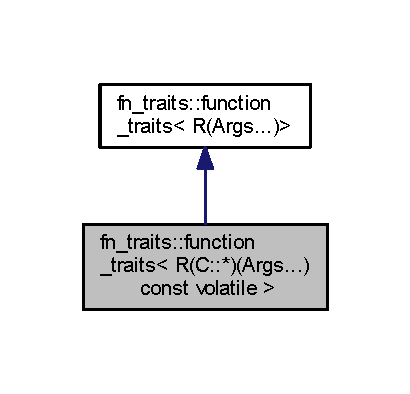
\includegraphics[width=197pt]{d3/d22/structfn__traits_1_1function__traits_3_01_r_07_c_1_1_5_08_07_args_8_8_8_08_01const_01volatile_01_4__inherit__graph}
\end{center}
\end{figure}


Collaboration diagram for fn\+\_\+traits\+:\+:function\+\_\+traits$<$ R(C\+:\+:$\ast$)(Args...) const volatile $>$\+:\nopagebreak
\begin{figure}[H]
\begin{center}
\leavevmode
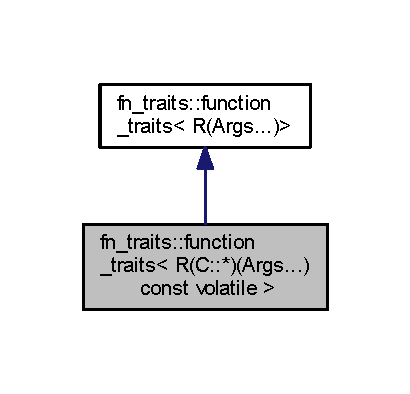
\includegraphics[width=197pt]{db/dc9/structfn__traits_1_1function__traits_3_01_r_07_c_1_1_5_08_07_args_8_8_8_08_01const_01volatile_01_4__coll__graph}
\end{center}
\end{figure}
\subsection*{Public Types}
\begin{DoxyCompactItemize}
\item 
typedef const volatile C \& \hyperlink{structfn__traits_1_1function__traits_3_01_r_07_c_1_1_5_08_07_args_8_8_8_08_01const_01volatile_01_4_ac9e0f1043d2bd54c554f14e2a05dfa0c}{owner\+\_\+type}
\item 
enum \{ \hyperlink{structfn__traits_1_1function__traits_3_01_r_07_args_8_8_8_08_4_aafde9521d9646c97b984646d8273dd3ba2f612b5524050ab8d6ab3d54d52dbbb0}{arity} = sizeof...( Args )
 \}
\item 
typedef R \hyperlink{structfn__traits_1_1function__traits_3_01_r_07_args_8_8_8_08_4_a1b509243ed1b4707465625de10e6c6bb}{result\+\_\+type}
\item 
typedef \hyperlink{structfn__traits_1_1function__traits_3_01_r_07_args_8_8_8_08_4_a1b509243ed1b4707465625de10e6c6bb}{result\+\_\+type} \hyperlink{structfn__traits_1_1function__traits_3_01_r_07_args_8_8_8_08_4_adf6a35a9b703dfb4778e59f132e00a9b}{return\+\_\+type}
\item 
typedef \hyperlink{structfn__traits_1_1function__traits_3_01_r_07_args_8_8_8_08_4_a1b509243ed1b4707465625de10e6c6bb}{result\+\_\+type} \hyperlink{structfn__traits_1_1function__traits_3_01_r_07_args_8_8_8_08_4_a85e5883a1c8050fe442c1072386b2d11}{function\+\_\+type}(Args...)
\item 
typedef std\+::tuple$<$ Args... $>$ \hyperlink{structfn__traits_1_1function__traits_3_01_r_07_args_8_8_8_08_4_a9b60ae8c79e52addf352e4ae7c8077b4}{tuple\+\_\+type}
\end{DoxyCompactItemize}


\subsection{Detailed Description}
\subsubsection*{template$<$typename C, typename R, typename... Args$>$\\*
struct fn\+\_\+traits\+::function\+\_\+traits$<$ R(\+C\+::$\ast$)(\+Args...) const volatile $>$}



Definition at line 64 of file function\+\_\+traits.\+hpp.



\subsection{Member Typedef Documentation}
\index{fn\+\_\+traits\+::function\+\_\+traits$<$ R(\+C\+::$\ast$)(\+Args...) const volatile $>$@{fn\+\_\+traits\+::function\+\_\+traits$<$ R(\+C\+::$\ast$)(\+Args...) const volatile $>$}!function\+\_\+type@{function\+\_\+type}}
\index{function\+\_\+type@{function\+\_\+type}!fn\+\_\+traits\+::function\+\_\+traits$<$ R(\+C\+::$\ast$)(\+Args...) const volatile $>$@{fn\+\_\+traits\+::function\+\_\+traits$<$ R(\+C\+::$\ast$)(\+Args...) const volatile $>$}}
\subsubsection[{\texorpdfstring{function\+\_\+type}{function_type}}]{\setlength{\rightskip}{0pt plus 5cm}template$<$typename R , typename... Args$>$ typedef {\bf result\+\_\+type} {\bf fn\+\_\+traits\+::function\+\_\+traits}$<$ R(Args...)$>$\+::function\+\_\+type(Args...)\hspace{0.3cm}{\ttfamily [inherited]}}\hypertarget{structfn__traits_1_1function__traits_3_01_r_07_args_8_8_8_08_4_a85e5883a1c8050fe442c1072386b2d11}{}\label{structfn__traits_1_1function__traits_3_01_r_07_args_8_8_8_08_4_a85e5883a1c8050fe442c1072386b2d11}


Definition at line 26 of file function\+\_\+traits.\+hpp.

\index{fn\+\_\+traits\+::function\+\_\+traits$<$ R(\+C\+::$\ast$)(\+Args...) const volatile $>$@{fn\+\_\+traits\+::function\+\_\+traits$<$ R(\+C\+::$\ast$)(\+Args...) const volatile $>$}!owner\+\_\+type@{owner\+\_\+type}}
\index{owner\+\_\+type@{owner\+\_\+type}!fn\+\_\+traits\+::function\+\_\+traits$<$ R(\+C\+::$\ast$)(\+Args...) const volatile $>$@{fn\+\_\+traits\+::function\+\_\+traits$<$ R(\+C\+::$\ast$)(\+Args...) const volatile $>$}}
\subsubsection[{\texorpdfstring{owner\+\_\+type}{owner_type}}]{\setlength{\rightskip}{0pt plus 5cm}template$<$typename C , typename R , typename... Args$>$ typedef const volatile C\& {\bf fn\+\_\+traits\+::function\+\_\+traits}$<$ R(C\+::$\ast$)(Args...) const volatile $>$\+::{\bf owner\+\_\+type}}\hypertarget{structfn__traits_1_1function__traits_3_01_r_07_c_1_1_5_08_07_args_8_8_8_08_01const_01volatile_01_4_ac9e0f1043d2bd54c554f14e2a05dfa0c}{}\label{structfn__traits_1_1function__traits_3_01_r_07_c_1_1_5_08_07_args_8_8_8_08_01const_01volatile_01_4_ac9e0f1043d2bd54c554f14e2a05dfa0c}


Definition at line 66 of file function\+\_\+traits.\+hpp.

\index{fn\+\_\+traits\+::function\+\_\+traits$<$ R(\+C\+::$\ast$)(\+Args...) const volatile $>$@{fn\+\_\+traits\+::function\+\_\+traits$<$ R(\+C\+::$\ast$)(\+Args...) const volatile $>$}!result\+\_\+type@{result\+\_\+type}}
\index{result\+\_\+type@{result\+\_\+type}!fn\+\_\+traits\+::function\+\_\+traits$<$ R(\+C\+::$\ast$)(\+Args...) const volatile $>$@{fn\+\_\+traits\+::function\+\_\+traits$<$ R(\+C\+::$\ast$)(\+Args...) const volatile $>$}}
\subsubsection[{\texorpdfstring{result\+\_\+type}{result_type}}]{\setlength{\rightskip}{0pt plus 5cm}template$<$typename R , typename... Args$>$ typedef R {\bf fn\+\_\+traits\+::function\+\_\+traits}$<$ R(Args...)$>$\+::{\bf result\+\_\+type}\hspace{0.3cm}{\ttfamily [inherited]}}\hypertarget{structfn__traits_1_1function__traits_3_01_r_07_args_8_8_8_08_4_a1b509243ed1b4707465625de10e6c6bb}{}\label{structfn__traits_1_1function__traits_3_01_r_07_args_8_8_8_08_4_a1b509243ed1b4707465625de10e6c6bb}


Definition at line 22 of file function\+\_\+traits.\+hpp.

\index{fn\+\_\+traits\+::function\+\_\+traits$<$ R(\+C\+::$\ast$)(\+Args...) const volatile $>$@{fn\+\_\+traits\+::function\+\_\+traits$<$ R(\+C\+::$\ast$)(\+Args...) const volatile $>$}!return\+\_\+type@{return\+\_\+type}}
\index{return\+\_\+type@{return\+\_\+type}!fn\+\_\+traits\+::function\+\_\+traits$<$ R(\+C\+::$\ast$)(\+Args...) const volatile $>$@{fn\+\_\+traits\+::function\+\_\+traits$<$ R(\+C\+::$\ast$)(\+Args...) const volatile $>$}}
\subsubsection[{\texorpdfstring{return\+\_\+type}{return_type}}]{\setlength{\rightskip}{0pt plus 5cm}template$<$typename R , typename... Args$>$ typedef {\bf result\+\_\+type} {\bf fn\+\_\+traits\+::function\+\_\+traits}$<$ R(Args...)$>$\+::{\bf return\+\_\+type}\hspace{0.3cm}{\ttfamily [inherited]}}\hypertarget{structfn__traits_1_1function__traits_3_01_r_07_args_8_8_8_08_4_adf6a35a9b703dfb4778e59f132e00a9b}{}\label{structfn__traits_1_1function__traits_3_01_r_07_args_8_8_8_08_4_adf6a35a9b703dfb4778e59f132e00a9b}


Definition at line 24 of file function\+\_\+traits.\+hpp.

\index{fn\+\_\+traits\+::function\+\_\+traits$<$ R(\+C\+::$\ast$)(\+Args...) const volatile $>$@{fn\+\_\+traits\+::function\+\_\+traits$<$ R(\+C\+::$\ast$)(\+Args...) const volatile $>$}!tuple\+\_\+type@{tuple\+\_\+type}}
\index{tuple\+\_\+type@{tuple\+\_\+type}!fn\+\_\+traits\+::function\+\_\+traits$<$ R(\+C\+::$\ast$)(\+Args...) const volatile $>$@{fn\+\_\+traits\+::function\+\_\+traits$<$ R(\+C\+::$\ast$)(\+Args...) const volatile $>$}}
\subsubsection[{\texorpdfstring{tuple\+\_\+type}{tuple_type}}]{\setlength{\rightskip}{0pt plus 5cm}template$<$typename R , typename... Args$>$ typedef std\+::tuple$<$Args...$>$ {\bf fn\+\_\+traits\+::function\+\_\+traits}$<$ R(Args...)$>$\+::{\bf tuple\+\_\+type}\hspace{0.3cm}{\ttfamily [inherited]}}\hypertarget{structfn__traits_1_1function__traits_3_01_r_07_args_8_8_8_08_4_a9b60ae8c79e52addf352e4ae7c8077b4}{}\label{structfn__traits_1_1function__traits_3_01_r_07_args_8_8_8_08_4_a9b60ae8c79e52addf352e4ae7c8077b4}


Definition at line 32 of file function\+\_\+traits.\+hpp.



\subsection{Member Enumeration Documentation}
\subsubsection[{\texorpdfstring{anonymous enum}{anonymous enum}}]{\setlength{\rightskip}{0pt plus 5cm}template$<$typename R , typename... Args$>$ anonymous enum\hspace{0.3cm}{\ttfamily [inherited]}}\hypertarget{structfn__traits_1_1function__traits_3_01_r_07_args_8_8_8_08_4_aafde9521d9646c97b984646d8273dd3b}{}\label{structfn__traits_1_1function__traits_3_01_r_07_args_8_8_8_08_4_aafde9521d9646c97b984646d8273dd3b}
\begin{Desc}
\item[Enumerator]\par
\begin{description}
\index{arity@{arity}!fn\+\_\+traits\+::function\+\_\+traits$<$ R(\+C\+::$\ast$)(\+Args...) const volatile $>$@{fn\+\_\+traits\+::function\+\_\+traits$<$ R(\+C\+::$\ast$)(\+Args...) const volatile $>$}}\index{fn\+\_\+traits\+::function\+\_\+traits$<$ R(\+C\+::$\ast$)(\+Args...) const volatile $>$@{fn\+\_\+traits\+::function\+\_\+traits$<$ R(\+C\+::$\ast$)(\+Args...) const volatile $>$}!arity@{arity}}\item[{\em 
arity\hypertarget{structfn__traits_1_1function__traits_3_01_r_07_args_8_8_8_08_4_aafde9521d9646c97b984646d8273dd3ba2f612b5524050ab8d6ab3d54d52dbbb0}{}\label{structfn__traits_1_1function__traits_3_01_r_07_args_8_8_8_08_4_aafde9521d9646c97b984646d8273dd3ba2f612b5524050ab8d6ab3d54d52dbbb0}
}]\end{description}
\end{Desc}


Definition at line 28 of file function\+\_\+traits.\+hpp.


\begin{DoxyCode}
28              \{
29             \hyperlink{structfn__traits_1_1function__traits_3_01_r_07_args_8_8_8_08_4_aafde9521d9646c97b984646d8273dd3ba2f612b5524050ab8d6ab3d54d52dbbb0}{arity} = \textcolor{keyword}{sizeof}...( Args )
30         \};
\end{DoxyCode}


The documentation for this struct was generated from the following file\+:\begin{DoxyCompactItemize}
\item 
include/\hyperlink{function__traits_8hpp}{function\+\_\+traits.\+hpp}\end{DoxyCompactItemize}

\hypertarget{structfn__traits_1_1function__traits_3_01_r_07_c_1_1_5_08_07_args_8_8_8_08_01volatile_01_4}{}\section{fn\+\_\+traits\+:\+:function\+\_\+traits$<$ R(C\+:\+:$\ast$)(Args...) volatile $>$ Struct Template Reference}
\label{structfn__traits_1_1function__traits_3_01_r_07_c_1_1_5_08_07_args_8_8_8_08_01volatile_01_4}\index{fn\+\_\+traits\+::function\+\_\+traits$<$ R(\+C\+::$\ast$)(\+Args...) volatile $>$@{fn\+\_\+traits\+::function\+\_\+traits$<$ R(\+C\+::$\ast$)(\+Args...) volatile $>$}}


{\ttfamily \#include $<$function\+\_\+traits.\+hpp$>$}



Inheritance diagram for fn\+\_\+traits\+:\+:function\+\_\+traits$<$ R(C\+:\+:$\ast$)(Args...) volatile $>$\+:\nopagebreak
\begin{figure}[H]
\begin{center}
\leavevmode
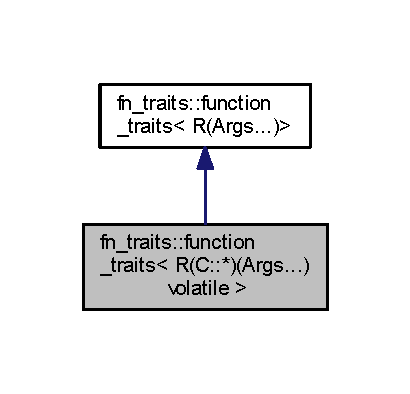
\includegraphics[width=197pt]{d9/d0d/structfn__traits_1_1function__traits_3_01_r_07_c_1_1_5_08_07_args_8_8_8_08_01volatile_01_4__inherit__graph}
\end{center}
\end{figure}


Collaboration diagram for fn\+\_\+traits\+:\+:function\+\_\+traits$<$ R(C\+:\+:$\ast$)(Args...) volatile $>$\+:\nopagebreak
\begin{figure}[H]
\begin{center}
\leavevmode
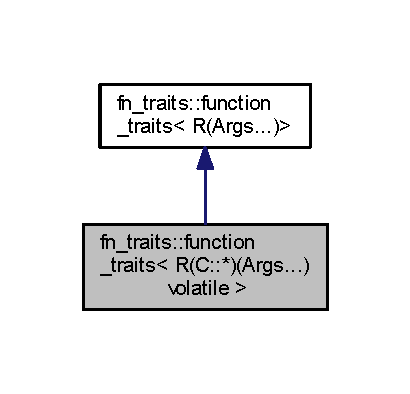
\includegraphics[width=197pt]{df/d53/structfn__traits_1_1function__traits_3_01_r_07_c_1_1_5_08_07_args_8_8_8_08_01volatile_01_4__coll__graph}
\end{center}
\end{figure}
\subsection*{Public Types}
\begin{DoxyCompactItemize}
\item 
typedef volatile C \& \hyperlink{structfn__traits_1_1function__traits_3_01_r_07_c_1_1_5_08_07_args_8_8_8_08_01volatile_01_4_a6dd56bc0e49730063f88ae55fd055a84}{owner\+\_\+type}
\item 
enum \{ \hyperlink{structfn__traits_1_1function__traits_3_01_r_07_args_8_8_8_08_4_aafde9521d9646c97b984646d8273dd3ba2f612b5524050ab8d6ab3d54d52dbbb0}{arity} = sizeof...( Args )
 \}
\item 
typedef R \hyperlink{structfn__traits_1_1function__traits_3_01_r_07_args_8_8_8_08_4_a1b509243ed1b4707465625de10e6c6bb}{result\+\_\+type}
\item 
typedef \hyperlink{structfn__traits_1_1function__traits_3_01_r_07_args_8_8_8_08_4_a1b509243ed1b4707465625de10e6c6bb}{result\+\_\+type} \hyperlink{structfn__traits_1_1function__traits_3_01_r_07_args_8_8_8_08_4_adf6a35a9b703dfb4778e59f132e00a9b}{return\+\_\+type}
\item 
typedef \hyperlink{structfn__traits_1_1function__traits_3_01_r_07_args_8_8_8_08_4_a1b509243ed1b4707465625de10e6c6bb}{result\+\_\+type} \hyperlink{structfn__traits_1_1function__traits_3_01_r_07_args_8_8_8_08_4_a85e5883a1c8050fe442c1072386b2d11}{function\+\_\+type}(Args...)
\item 
typedef std\+::tuple$<$ Args... $>$ \hyperlink{structfn__traits_1_1function__traits_3_01_r_07_args_8_8_8_08_4_a9b60ae8c79e52addf352e4ae7c8077b4}{tuple\+\_\+type}
\end{DoxyCompactItemize}


\subsection{Detailed Description}
\subsubsection*{template$<$typename C, typename R, typename... Args$>$\\*
struct fn\+\_\+traits\+::function\+\_\+traits$<$ R(\+C\+::$\ast$)(\+Args...) volatile $>$}



Definition at line 58 of file function\+\_\+traits.\+hpp.



\subsection{Member Typedef Documentation}
\index{fn\+\_\+traits\+::function\+\_\+traits$<$ R(\+C\+::$\ast$)(\+Args...) volatile $>$@{fn\+\_\+traits\+::function\+\_\+traits$<$ R(\+C\+::$\ast$)(\+Args...) volatile $>$}!function\+\_\+type@{function\+\_\+type}}
\index{function\+\_\+type@{function\+\_\+type}!fn\+\_\+traits\+::function\+\_\+traits$<$ R(\+C\+::$\ast$)(\+Args...) volatile $>$@{fn\+\_\+traits\+::function\+\_\+traits$<$ R(\+C\+::$\ast$)(\+Args...) volatile $>$}}
\subsubsection[{\texorpdfstring{function\+\_\+type}{function_type}}]{\setlength{\rightskip}{0pt plus 5cm}template$<$typename R , typename... Args$>$ typedef {\bf result\+\_\+type} {\bf fn\+\_\+traits\+::function\+\_\+traits}$<$ R(Args...)$>$\+::function\+\_\+type(Args...)\hspace{0.3cm}{\ttfamily [inherited]}}\hypertarget{structfn__traits_1_1function__traits_3_01_r_07_args_8_8_8_08_4_a85e5883a1c8050fe442c1072386b2d11}{}\label{structfn__traits_1_1function__traits_3_01_r_07_args_8_8_8_08_4_a85e5883a1c8050fe442c1072386b2d11}


Definition at line 26 of file function\+\_\+traits.\+hpp.

\index{fn\+\_\+traits\+::function\+\_\+traits$<$ R(\+C\+::$\ast$)(\+Args...) volatile $>$@{fn\+\_\+traits\+::function\+\_\+traits$<$ R(\+C\+::$\ast$)(\+Args...) volatile $>$}!owner\+\_\+type@{owner\+\_\+type}}
\index{owner\+\_\+type@{owner\+\_\+type}!fn\+\_\+traits\+::function\+\_\+traits$<$ R(\+C\+::$\ast$)(\+Args...) volatile $>$@{fn\+\_\+traits\+::function\+\_\+traits$<$ R(\+C\+::$\ast$)(\+Args...) volatile $>$}}
\subsubsection[{\texorpdfstring{owner\+\_\+type}{owner_type}}]{\setlength{\rightskip}{0pt plus 5cm}template$<$typename C , typename R , typename... Args$>$ typedef volatile C\& {\bf fn\+\_\+traits\+::function\+\_\+traits}$<$ R(C\+::$\ast$)(Args...) volatile $>$\+::{\bf owner\+\_\+type}}\hypertarget{structfn__traits_1_1function__traits_3_01_r_07_c_1_1_5_08_07_args_8_8_8_08_01volatile_01_4_a6dd56bc0e49730063f88ae55fd055a84}{}\label{structfn__traits_1_1function__traits_3_01_r_07_c_1_1_5_08_07_args_8_8_8_08_01volatile_01_4_a6dd56bc0e49730063f88ae55fd055a84}


Definition at line 60 of file function\+\_\+traits.\+hpp.

\index{fn\+\_\+traits\+::function\+\_\+traits$<$ R(\+C\+::$\ast$)(\+Args...) volatile $>$@{fn\+\_\+traits\+::function\+\_\+traits$<$ R(\+C\+::$\ast$)(\+Args...) volatile $>$}!result\+\_\+type@{result\+\_\+type}}
\index{result\+\_\+type@{result\+\_\+type}!fn\+\_\+traits\+::function\+\_\+traits$<$ R(\+C\+::$\ast$)(\+Args...) volatile $>$@{fn\+\_\+traits\+::function\+\_\+traits$<$ R(\+C\+::$\ast$)(\+Args...) volatile $>$}}
\subsubsection[{\texorpdfstring{result\+\_\+type}{result_type}}]{\setlength{\rightskip}{0pt plus 5cm}template$<$typename R , typename... Args$>$ typedef R {\bf fn\+\_\+traits\+::function\+\_\+traits}$<$ R(Args...)$>$\+::{\bf result\+\_\+type}\hspace{0.3cm}{\ttfamily [inherited]}}\hypertarget{structfn__traits_1_1function__traits_3_01_r_07_args_8_8_8_08_4_a1b509243ed1b4707465625de10e6c6bb}{}\label{structfn__traits_1_1function__traits_3_01_r_07_args_8_8_8_08_4_a1b509243ed1b4707465625de10e6c6bb}


Definition at line 22 of file function\+\_\+traits.\+hpp.

\index{fn\+\_\+traits\+::function\+\_\+traits$<$ R(\+C\+::$\ast$)(\+Args...) volatile $>$@{fn\+\_\+traits\+::function\+\_\+traits$<$ R(\+C\+::$\ast$)(\+Args...) volatile $>$}!return\+\_\+type@{return\+\_\+type}}
\index{return\+\_\+type@{return\+\_\+type}!fn\+\_\+traits\+::function\+\_\+traits$<$ R(\+C\+::$\ast$)(\+Args...) volatile $>$@{fn\+\_\+traits\+::function\+\_\+traits$<$ R(\+C\+::$\ast$)(\+Args...) volatile $>$}}
\subsubsection[{\texorpdfstring{return\+\_\+type}{return_type}}]{\setlength{\rightskip}{0pt plus 5cm}template$<$typename R , typename... Args$>$ typedef {\bf result\+\_\+type} {\bf fn\+\_\+traits\+::function\+\_\+traits}$<$ R(Args...)$>$\+::{\bf return\+\_\+type}\hspace{0.3cm}{\ttfamily [inherited]}}\hypertarget{structfn__traits_1_1function__traits_3_01_r_07_args_8_8_8_08_4_adf6a35a9b703dfb4778e59f132e00a9b}{}\label{structfn__traits_1_1function__traits_3_01_r_07_args_8_8_8_08_4_adf6a35a9b703dfb4778e59f132e00a9b}


Definition at line 24 of file function\+\_\+traits.\+hpp.

\index{fn\+\_\+traits\+::function\+\_\+traits$<$ R(\+C\+::$\ast$)(\+Args...) volatile $>$@{fn\+\_\+traits\+::function\+\_\+traits$<$ R(\+C\+::$\ast$)(\+Args...) volatile $>$}!tuple\+\_\+type@{tuple\+\_\+type}}
\index{tuple\+\_\+type@{tuple\+\_\+type}!fn\+\_\+traits\+::function\+\_\+traits$<$ R(\+C\+::$\ast$)(\+Args...) volatile $>$@{fn\+\_\+traits\+::function\+\_\+traits$<$ R(\+C\+::$\ast$)(\+Args...) volatile $>$}}
\subsubsection[{\texorpdfstring{tuple\+\_\+type}{tuple_type}}]{\setlength{\rightskip}{0pt plus 5cm}template$<$typename R , typename... Args$>$ typedef std\+::tuple$<$Args...$>$ {\bf fn\+\_\+traits\+::function\+\_\+traits}$<$ R(Args...)$>$\+::{\bf tuple\+\_\+type}\hspace{0.3cm}{\ttfamily [inherited]}}\hypertarget{structfn__traits_1_1function__traits_3_01_r_07_args_8_8_8_08_4_a9b60ae8c79e52addf352e4ae7c8077b4}{}\label{structfn__traits_1_1function__traits_3_01_r_07_args_8_8_8_08_4_a9b60ae8c79e52addf352e4ae7c8077b4}


Definition at line 32 of file function\+\_\+traits.\+hpp.



\subsection{Member Enumeration Documentation}
\subsubsection[{\texorpdfstring{anonymous enum}{anonymous enum}}]{\setlength{\rightskip}{0pt plus 5cm}template$<$typename R , typename... Args$>$ anonymous enum\hspace{0.3cm}{\ttfamily [inherited]}}\hypertarget{structfn__traits_1_1function__traits_3_01_r_07_args_8_8_8_08_4_aafde9521d9646c97b984646d8273dd3b}{}\label{structfn__traits_1_1function__traits_3_01_r_07_args_8_8_8_08_4_aafde9521d9646c97b984646d8273dd3b}
\begin{Desc}
\item[Enumerator]\par
\begin{description}
\index{arity@{arity}!fn\+\_\+traits\+::function\+\_\+traits$<$ R(\+C\+::$\ast$)(\+Args...) volatile $>$@{fn\+\_\+traits\+::function\+\_\+traits$<$ R(\+C\+::$\ast$)(\+Args...) volatile $>$}}\index{fn\+\_\+traits\+::function\+\_\+traits$<$ R(\+C\+::$\ast$)(\+Args...) volatile $>$@{fn\+\_\+traits\+::function\+\_\+traits$<$ R(\+C\+::$\ast$)(\+Args...) volatile $>$}!arity@{arity}}\item[{\em 
arity\hypertarget{structfn__traits_1_1function__traits_3_01_r_07_args_8_8_8_08_4_aafde9521d9646c97b984646d8273dd3ba2f612b5524050ab8d6ab3d54d52dbbb0}{}\label{structfn__traits_1_1function__traits_3_01_r_07_args_8_8_8_08_4_aafde9521d9646c97b984646d8273dd3ba2f612b5524050ab8d6ab3d54d52dbbb0}
}]\end{description}
\end{Desc}


Definition at line 28 of file function\+\_\+traits.\+hpp.


\begin{DoxyCode}
28              \{
29             \hyperlink{structfn__traits_1_1function__traits_3_01_r_07_args_8_8_8_08_4_aafde9521d9646c97b984646d8273dd3ba2f612b5524050ab8d6ab3d54d52dbbb0}{arity} = \textcolor{keyword}{sizeof}...( Args )
30         \};
\end{DoxyCode}


The documentation for this struct was generated from the following file\+:\begin{DoxyCompactItemize}
\item 
include/\hyperlink{function__traits_8hpp}{function\+\_\+traits.\+hpp}\end{DoxyCompactItemize}

\hypertarget{structfn__traits_1_1function__traits_3_01_r_07_c_1_1_5_08_07_args_8_8_8_08_4}{}\section{fn\+\_\+traits\+:\+:function\+\_\+traits$<$ R(C\+:\+:$\ast$)(Args...)$>$ Struct Template Reference}
\label{structfn__traits_1_1function__traits_3_01_r_07_c_1_1_5_08_07_args_8_8_8_08_4}\index{fn\+\_\+traits\+::function\+\_\+traits$<$ R(\+C\+::$\ast$)(\+Args...)$>$@{fn\+\_\+traits\+::function\+\_\+traits$<$ R(\+C\+::$\ast$)(\+Args...)$>$}}


{\ttfamily \#include $<$function\+\_\+traits.\+hpp$>$}



Inheritance diagram for fn\+\_\+traits\+:\+:function\+\_\+traits$<$ R(C\+:\+:$\ast$)(Args...)$>$\+:\nopagebreak
\begin{figure}[H]
\begin{center}
\leavevmode
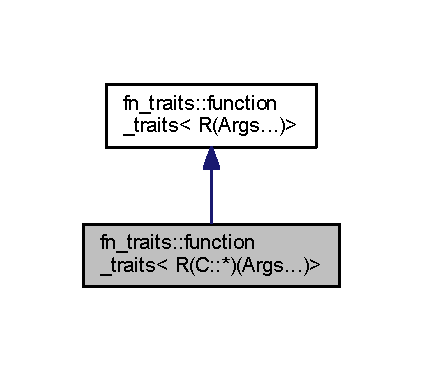
\includegraphics[width=203pt]{d8/df2/structfn__traits_1_1function__traits_3_01_r_07_c_1_1_5_08_07_args_8_8_8_08_4__inherit__graph}
\end{center}
\end{figure}


Collaboration diagram for fn\+\_\+traits\+:\+:function\+\_\+traits$<$ R(C\+:\+:$\ast$)(Args...)$>$\+:\nopagebreak
\begin{figure}[H]
\begin{center}
\leavevmode
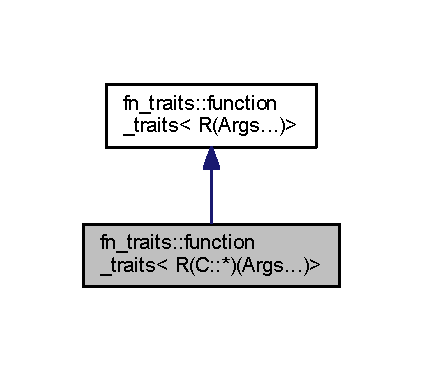
\includegraphics[width=203pt]{d3/d96/structfn__traits_1_1function__traits_3_01_r_07_c_1_1_5_08_07_args_8_8_8_08_4__coll__graph}
\end{center}
\end{figure}
\subsection*{Public Types}
\begin{DoxyCompactItemize}
\item 
typedef C \& \hyperlink{structfn__traits_1_1function__traits_3_01_r_07_c_1_1_5_08_07_args_8_8_8_08_4_aa6e7fe5af891f86ccb332181422c219d}{owner\+\_\+type}
\item 
enum \{ \hyperlink{structfn__traits_1_1function__traits_3_01_r_07_args_8_8_8_08_4_aafde9521d9646c97b984646d8273dd3ba2f612b5524050ab8d6ab3d54d52dbbb0}{arity} = sizeof...( Args )
 \}
\item 
typedef R \hyperlink{structfn__traits_1_1function__traits_3_01_r_07_args_8_8_8_08_4_a1b509243ed1b4707465625de10e6c6bb}{result\+\_\+type}
\item 
typedef \hyperlink{structfn__traits_1_1function__traits_3_01_r_07_args_8_8_8_08_4_a1b509243ed1b4707465625de10e6c6bb}{result\+\_\+type} \hyperlink{structfn__traits_1_1function__traits_3_01_r_07_args_8_8_8_08_4_adf6a35a9b703dfb4778e59f132e00a9b}{return\+\_\+type}
\item 
typedef \hyperlink{structfn__traits_1_1function__traits_3_01_r_07_args_8_8_8_08_4_a1b509243ed1b4707465625de10e6c6bb}{result\+\_\+type} \hyperlink{structfn__traits_1_1function__traits_3_01_r_07_args_8_8_8_08_4_a85e5883a1c8050fe442c1072386b2d11}{function\+\_\+type}(Args...)
\item 
typedef std\+::tuple$<$ Args... $>$ \hyperlink{structfn__traits_1_1function__traits_3_01_r_07_args_8_8_8_08_4_a9b60ae8c79e52addf352e4ae7c8077b4}{tuple\+\_\+type}
\end{DoxyCompactItemize}


\subsection{Detailed Description}
\subsubsection*{template$<$typename C, typename R, typename... Args$>$\\*
struct fn\+\_\+traits\+::function\+\_\+traits$<$ R(\+C\+::$\ast$)(\+Args...)$>$}



Definition at line 46 of file function\+\_\+traits.\+hpp.



\subsection{Member Typedef Documentation}
\index{fn\+\_\+traits\+::function\+\_\+traits$<$ R(\+C\+::$\ast$)(\+Args...)$>$@{fn\+\_\+traits\+::function\+\_\+traits$<$ R(\+C\+::$\ast$)(\+Args...)$>$}!function\+\_\+type@{function\+\_\+type}}
\index{function\+\_\+type@{function\+\_\+type}!fn\+\_\+traits\+::function\+\_\+traits$<$ R(\+C\+::$\ast$)(\+Args...)$>$@{fn\+\_\+traits\+::function\+\_\+traits$<$ R(\+C\+::$\ast$)(\+Args...)$>$}}
\subsubsection[{\texorpdfstring{function\+\_\+type}{function_type}}]{\setlength{\rightskip}{0pt plus 5cm}template$<$typename R , typename... Args$>$ typedef {\bf result\+\_\+type} {\bf fn\+\_\+traits\+::function\+\_\+traits}$<$ R(Args...)$>$\+::function\+\_\+type(Args...)\hspace{0.3cm}{\ttfamily [inherited]}}\hypertarget{structfn__traits_1_1function__traits_3_01_r_07_args_8_8_8_08_4_a85e5883a1c8050fe442c1072386b2d11}{}\label{structfn__traits_1_1function__traits_3_01_r_07_args_8_8_8_08_4_a85e5883a1c8050fe442c1072386b2d11}


Definition at line 26 of file function\+\_\+traits.\+hpp.

\index{fn\+\_\+traits\+::function\+\_\+traits$<$ R(\+C\+::$\ast$)(\+Args...)$>$@{fn\+\_\+traits\+::function\+\_\+traits$<$ R(\+C\+::$\ast$)(\+Args...)$>$}!owner\+\_\+type@{owner\+\_\+type}}
\index{owner\+\_\+type@{owner\+\_\+type}!fn\+\_\+traits\+::function\+\_\+traits$<$ R(\+C\+::$\ast$)(\+Args...)$>$@{fn\+\_\+traits\+::function\+\_\+traits$<$ R(\+C\+::$\ast$)(\+Args...)$>$}}
\subsubsection[{\texorpdfstring{owner\+\_\+type}{owner_type}}]{\setlength{\rightskip}{0pt plus 5cm}template$<$typename C , typename R , typename... Args$>$ typedef C\& {\bf fn\+\_\+traits\+::function\+\_\+traits}$<$ R(C\+::$\ast$)(Args...)$>$\+::{\bf owner\+\_\+type}}\hypertarget{structfn__traits_1_1function__traits_3_01_r_07_c_1_1_5_08_07_args_8_8_8_08_4_aa6e7fe5af891f86ccb332181422c219d}{}\label{structfn__traits_1_1function__traits_3_01_r_07_c_1_1_5_08_07_args_8_8_8_08_4_aa6e7fe5af891f86ccb332181422c219d}


Definition at line 48 of file function\+\_\+traits.\+hpp.

\index{fn\+\_\+traits\+::function\+\_\+traits$<$ R(\+C\+::$\ast$)(\+Args...)$>$@{fn\+\_\+traits\+::function\+\_\+traits$<$ R(\+C\+::$\ast$)(\+Args...)$>$}!result\+\_\+type@{result\+\_\+type}}
\index{result\+\_\+type@{result\+\_\+type}!fn\+\_\+traits\+::function\+\_\+traits$<$ R(\+C\+::$\ast$)(\+Args...)$>$@{fn\+\_\+traits\+::function\+\_\+traits$<$ R(\+C\+::$\ast$)(\+Args...)$>$}}
\subsubsection[{\texorpdfstring{result\+\_\+type}{result_type}}]{\setlength{\rightskip}{0pt plus 5cm}template$<$typename R , typename... Args$>$ typedef R {\bf fn\+\_\+traits\+::function\+\_\+traits}$<$ R(Args...)$>$\+::{\bf result\+\_\+type}\hspace{0.3cm}{\ttfamily [inherited]}}\hypertarget{structfn__traits_1_1function__traits_3_01_r_07_args_8_8_8_08_4_a1b509243ed1b4707465625de10e6c6bb}{}\label{structfn__traits_1_1function__traits_3_01_r_07_args_8_8_8_08_4_a1b509243ed1b4707465625de10e6c6bb}


Definition at line 22 of file function\+\_\+traits.\+hpp.

\index{fn\+\_\+traits\+::function\+\_\+traits$<$ R(\+C\+::$\ast$)(\+Args...)$>$@{fn\+\_\+traits\+::function\+\_\+traits$<$ R(\+C\+::$\ast$)(\+Args...)$>$}!return\+\_\+type@{return\+\_\+type}}
\index{return\+\_\+type@{return\+\_\+type}!fn\+\_\+traits\+::function\+\_\+traits$<$ R(\+C\+::$\ast$)(\+Args...)$>$@{fn\+\_\+traits\+::function\+\_\+traits$<$ R(\+C\+::$\ast$)(\+Args...)$>$}}
\subsubsection[{\texorpdfstring{return\+\_\+type}{return_type}}]{\setlength{\rightskip}{0pt plus 5cm}template$<$typename R , typename... Args$>$ typedef {\bf result\+\_\+type} {\bf fn\+\_\+traits\+::function\+\_\+traits}$<$ R(Args...)$>$\+::{\bf return\+\_\+type}\hspace{0.3cm}{\ttfamily [inherited]}}\hypertarget{structfn__traits_1_1function__traits_3_01_r_07_args_8_8_8_08_4_adf6a35a9b703dfb4778e59f132e00a9b}{}\label{structfn__traits_1_1function__traits_3_01_r_07_args_8_8_8_08_4_adf6a35a9b703dfb4778e59f132e00a9b}


Definition at line 24 of file function\+\_\+traits.\+hpp.

\index{fn\+\_\+traits\+::function\+\_\+traits$<$ R(\+C\+::$\ast$)(\+Args...)$>$@{fn\+\_\+traits\+::function\+\_\+traits$<$ R(\+C\+::$\ast$)(\+Args...)$>$}!tuple\+\_\+type@{tuple\+\_\+type}}
\index{tuple\+\_\+type@{tuple\+\_\+type}!fn\+\_\+traits\+::function\+\_\+traits$<$ R(\+C\+::$\ast$)(\+Args...)$>$@{fn\+\_\+traits\+::function\+\_\+traits$<$ R(\+C\+::$\ast$)(\+Args...)$>$}}
\subsubsection[{\texorpdfstring{tuple\+\_\+type}{tuple_type}}]{\setlength{\rightskip}{0pt plus 5cm}template$<$typename R , typename... Args$>$ typedef std\+::tuple$<$Args...$>$ {\bf fn\+\_\+traits\+::function\+\_\+traits}$<$ R(Args...)$>$\+::{\bf tuple\+\_\+type}\hspace{0.3cm}{\ttfamily [inherited]}}\hypertarget{structfn__traits_1_1function__traits_3_01_r_07_args_8_8_8_08_4_a9b60ae8c79e52addf352e4ae7c8077b4}{}\label{structfn__traits_1_1function__traits_3_01_r_07_args_8_8_8_08_4_a9b60ae8c79e52addf352e4ae7c8077b4}


Definition at line 32 of file function\+\_\+traits.\+hpp.



\subsection{Member Enumeration Documentation}
\subsubsection[{\texorpdfstring{anonymous enum}{anonymous enum}}]{\setlength{\rightskip}{0pt plus 5cm}template$<$typename R , typename... Args$>$ anonymous enum\hspace{0.3cm}{\ttfamily [inherited]}}\hypertarget{structfn__traits_1_1function__traits_3_01_r_07_args_8_8_8_08_4_aafde9521d9646c97b984646d8273dd3b}{}\label{structfn__traits_1_1function__traits_3_01_r_07_args_8_8_8_08_4_aafde9521d9646c97b984646d8273dd3b}
\begin{Desc}
\item[Enumerator]\par
\begin{description}
\index{arity@{arity}!fn\+\_\+traits\+::function\+\_\+traits$<$ R(\+C\+::$\ast$)(\+Args...)$>$@{fn\+\_\+traits\+::function\+\_\+traits$<$ R(\+C\+::$\ast$)(\+Args...)$>$}}\index{fn\+\_\+traits\+::function\+\_\+traits$<$ R(\+C\+::$\ast$)(\+Args...)$>$@{fn\+\_\+traits\+::function\+\_\+traits$<$ R(\+C\+::$\ast$)(\+Args...)$>$}!arity@{arity}}\item[{\em 
arity\hypertarget{structfn__traits_1_1function__traits_3_01_r_07_args_8_8_8_08_4_aafde9521d9646c97b984646d8273dd3ba2f612b5524050ab8d6ab3d54d52dbbb0}{}\label{structfn__traits_1_1function__traits_3_01_r_07_args_8_8_8_08_4_aafde9521d9646c97b984646d8273dd3ba2f612b5524050ab8d6ab3d54d52dbbb0}
}]\end{description}
\end{Desc}


Definition at line 28 of file function\+\_\+traits.\+hpp.


\begin{DoxyCode}
28              \{
29             \hyperlink{structfn__traits_1_1function__traits_3_01_r_07_args_8_8_8_08_4_aafde9521d9646c97b984646d8273dd3ba2f612b5524050ab8d6ab3d54d52dbbb0}{arity} = \textcolor{keyword}{sizeof}...( Args )
30         \};
\end{DoxyCode}


The documentation for this struct was generated from the following file\+:\begin{DoxyCompactItemize}
\item 
include/\hyperlink{function__traits_8hpp}{function\+\_\+traits.\+hpp}\end{DoxyCompactItemize}

\hypertarget{structfn__traits_1_1function__traits_3_01std_1_1function_3_01_functor_01_4_01_4}{}\section{fn\+\_\+traits\+:\+:function\+\_\+traits$<$ std\+:\+:function$<$ Functor $>$ $>$ Struct Template Reference}
\label{structfn__traits_1_1function__traits_3_01std_1_1function_3_01_functor_01_4_01_4}\index{fn\+\_\+traits\+::function\+\_\+traits$<$ std\+::function$<$ Functor $>$ $>$@{fn\+\_\+traits\+::function\+\_\+traits$<$ std\+::function$<$ Functor $>$ $>$}}


{\ttfamily \#include $<$function\+\_\+traits.\+hpp$>$}



Inheritance diagram for fn\+\_\+traits\+:\+:function\+\_\+traits$<$ std\+:\+:function$<$ Functor $>$ $>$\+:\nopagebreak
\begin{figure}[H]
\begin{center}
\leavevmode
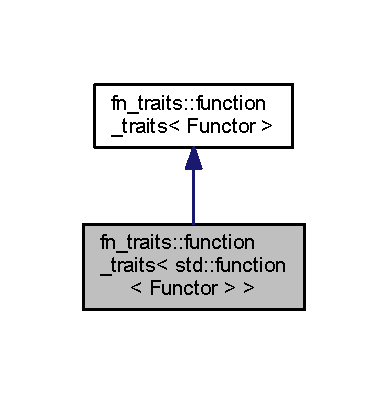
\includegraphics[width=186pt]{dc/df7/structfn__traits_1_1function__traits_3_01std_1_1function_3_01_functor_01_4_01_4__inherit__graph}
\end{center}
\end{figure}


Collaboration diagram for fn\+\_\+traits\+:\+:function\+\_\+traits$<$ std\+:\+:function$<$ Functor $>$ $>$\+:\nopagebreak
\begin{figure}[H]
\begin{center}
\leavevmode
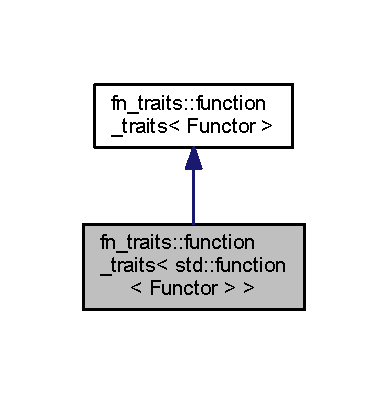
\includegraphics[width=186pt]{d4/d3f/structfn__traits_1_1function__traits_3_01std_1_1function_3_01_functor_01_4_01_4__coll__graph}
\end{center}
\end{figure}


\subsection{Detailed Description}
\subsubsection*{template$<$typename Functor$>$\\*
struct fn\+\_\+traits\+::function\+\_\+traits$<$ std\+::function$<$ Functor $>$ $>$}



Definition at line 109 of file function\+\_\+traits.\+hpp.



The documentation for this struct was generated from the following file\+:\begin{DoxyCompactItemize}
\item 
include/\hyperlink{function__traits_8hpp}{function\+\_\+traits.\+hpp}\end{DoxyCompactItemize}

\hypertarget{structfn__traits_1_1function__traits_3_01_t_01_6_01_4}{}\section{fn\+\_\+traits\+:\+:function\+\_\+traits$<$ T \& $>$ Struct Template Reference}
\label{structfn__traits_1_1function__traits_3_01_t_01_6_01_4}\index{fn\+\_\+traits\+::function\+\_\+traits$<$ T \& $>$@{fn\+\_\+traits\+::function\+\_\+traits$<$ T \& $>$}}


{\ttfamily \#include $<$function\+\_\+traits.\+hpp$>$}



Inheritance diagram for fn\+\_\+traits\+:\+:function\+\_\+traits$<$ T \& $>$\+:\nopagebreak
\begin{figure}[H]
\begin{center}
\leavevmode
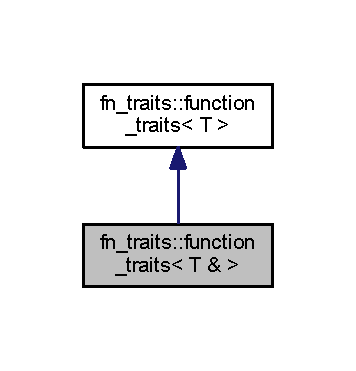
\includegraphics[width=171pt]{db/d2b/structfn__traits_1_1function__traits_3_01_t_01_6_01_4__inherit__graph}
\end{center}
\end{figure}


Collaboration diagram for fn\+\_\+traits\+:\+:function\+\_\+traits$<$ T \& $>$\+:\nopagebreak
\begin{figure}[H]
\begin{center}
\leavevmode
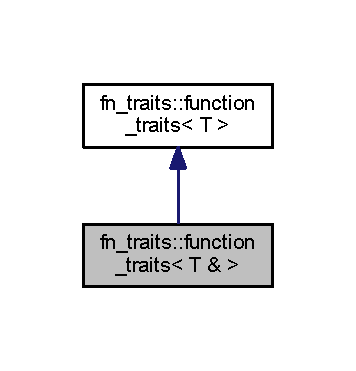
\includegraphics[width=171pt]{d3/d91/structfn__traits_1_1function__traits_3_01_t_01_6_01_4__coll__graph}
\end{center}
\end{figure}


\subsection{Detailed Description}
\subsubsection*{template$<$typename T$>$\\*
struct fn\+\_\+traits\+::function\+\_\+traits$<$ T \& $>$}



Definition at line 114 of file function\+\_\+traits.\+hpp.



The documentation for this struct was generated from the following file\+:\begin{DoxyCompactItemize}
\item 
include/\hyperlink{function__traits_8hpp}{function\+\_\+traits.\+hpp}\end{DoxyCompactItemize}

\hypertarget{structfn__traits_1_1function__traits_3_01_t_01_6_6_01_4}{}\section{fn\+\_\+traits\+:\+:function\+\_\+traits$<$ T \&\& $>$ Struct Template Reference}
\label{structfn__traits_1_1function__traits_3_01_t_01_6_6_01_4}\index{fn\+\_\+traits\+::function\+\_\+traits$<$ T \&\& $>$@{fn\+\_\+traits\+::function\+\_\+traits$<$ T \&\& $>$}}


{\ttfamily \#include $<$function\+\_\+traits.\+hpp$>$}



Inheritance diagram for fn\+\_\+traits\+:\+:function\+\_\+traits$<$ T \&\& $>$\+:\nopagebreak
\begin{figure}[H]
\begin{center}
\leavevmode
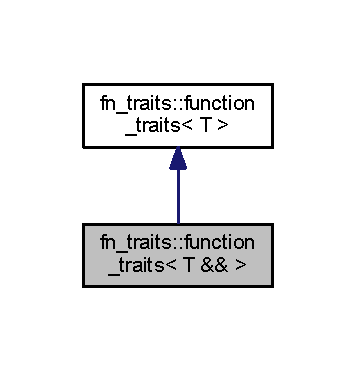
\includegraphics[width=171pt]{db/dfd/structfn__traits_1_1function__traits_3_01_t_01_6_6_01_4__inherit__graph}
\end{center}
\end{figure}


Collaboration diagram for fn\+\_\+traits\+:\+:function\+\_\+traits$<$ T \&\& $>$\+:\nopagebreak
\begin{figure}[H]
\begin{center}
\leavevmode
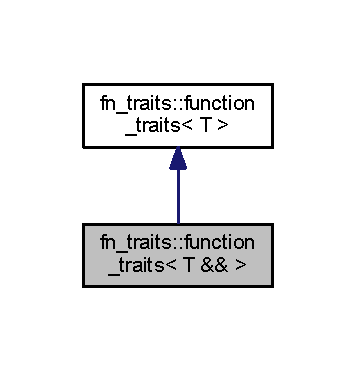
\includegraphics[width=171pt]{d4/d35/structfn__traits_1_1function__traits_3_01_t_01_6_6_01_4__coll__graph}
\end{center}
\end{figure}


\subsection{Detailed Description}
\subsubsection*{template$<$typename T$>$\\*
struct fn\+\_\+traits\+::function\+\_\+traits$<$ T \&\& $>$}



Definition at line 130 of file function\+\_\+traits.\+hpp.



The documentation for this struct was generated from the following file\+:\begin{DoxyCompactItemize}
\item 
include/\hyperlink{function__traits_8hpp}{function\+\_\+traits.\+hpp}\end{DoxyCompactItemize}

\hypertarget{structfn__traits_1_1function__traits_3_01volatile_01_t_01_6_01_4}{}\section{fn\+\_\+traits\+:\+:function\+\_\+traits$<$ volatile T \& $>$ Struct Template Reference}
\label{structfn__traits_1_1function__traits_3_01volatile_01_t_01_6_01_4}\index{fn\+\_\+traits\+::function\+\_\+traits$<$ volatile T \& $>$@{fn\+\_\+traits\+::function\+\_\+traits$<$ volatile T \& $>$}}


{\ttfamily \#include $<$function\+\_\+traits.\+hpp$>$}



Inheritance diagram for fn\+\_\+traits\+:\+:function\+\_\+traits$<$ volatile T \& $>$\+:\nopagebreak
\begin{figure}[H]
\begin{center}
\leavevmode
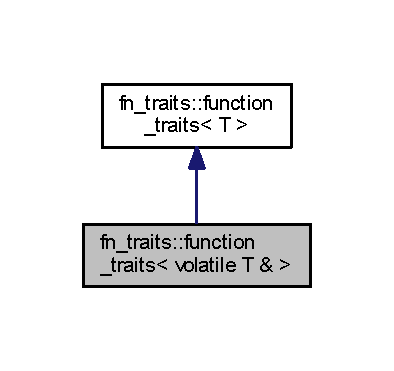
\includegraphics[width=189pt]{da/d1b/structfn__traits_1_1function__traits_3_01volatile_01_t_01_6_01_4__inherit__graph}
\end{center}
\end{figure}


Collaboration diagram for fn\+\_\+traits\+:\+:function\+\_\+traits$<$ volatile T \& $>$\+:\nopagebreak
\begin{figure}[H]
\begin{center}
\leavevmode
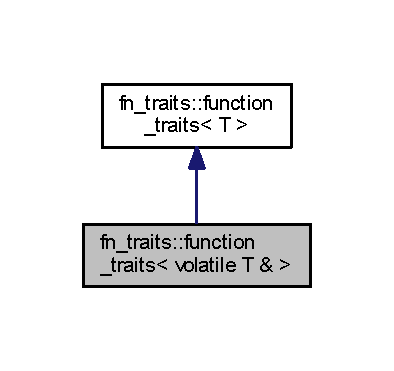
\includegraphics[width=189pt]{d2/d51/structfn__traits_1_1function__traits_3_01volatile_01_t_01_6_01_4__coll__graph}
\end{center}
\end{figure}


\subsection{Detailed Description}
\subsubsection*{template$<$typename T$>$\\*
struct fn\+\_\+traits\+::function\+\_\+traits$<$ volatile T \& $>$}



Definition at line 122 of file function\+\_\+traits.\+hpp.



The documentation for this struct was generated from the following file\+:\begin{DoxyCompactItemize}
\item 
include/\hyperlink{function__traits_8hpp}{function\+\_\+traits.\+hpp}\end{DoxyCompactItemize}

\hypertarget{structfn__traits_1_1function__traits_3_01volatile_01_t_01_6_6_01_4}{}\section{fn\+\_\+traits\+:\+:function\+\_\+traits$<$ volatile T \&\& $>$ Struct Template Reference}
\label{structfn__traits_1_1function__traits_3_01volatile_01_t_01_6_6_01_4}\index{fn\+\_\+traits\+::function\+\_\+traits$<$ volatile T \&\& $>$@{fn\+\_\+traits\+::function\+\_\+traits$<$ volatile T \&\& $>$}}


{\ttfamily \#include $<$function\+\_\+traits.\+hpp$>$}



Inheritance diagram for fn\+\_\+traits\+:\+:function\+\_\+traits$<$ volatile T \&\& $>$\+:\nopagebreak
\begin{figure}[H]
\begin{center}
\leavevmode
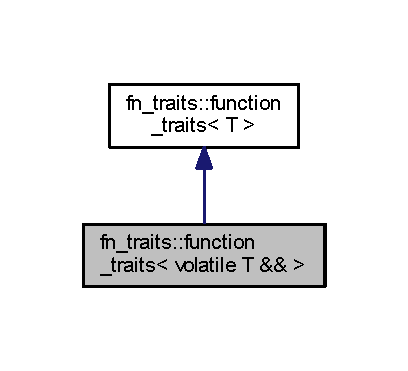
\includegraphics[width=196pt]{dd/db4/structfn__traits_1_1function__traits_3_01volatile_01_t_01_6_6_01_4__inherit__graph}
\end{center}
\end{figure}


Collaboration diagram for fn\+\_\+traits\+:\+:function\+\_\+traits$<$ volatile T \&\& $>$\+:\nopagebreak
\begin{figure}[H]
\begin{center}
\leavevmode
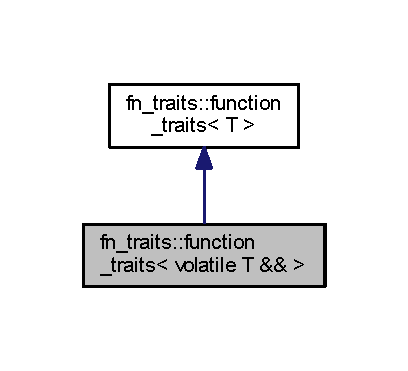
\includegraphics[width=196pt]{d8/dac/structfn__traits_1_1function__traits_3_01volatile_01_t_01_6_6_01_4__coll__graph}
\end{center}
\end{figure}


\subsection{Detailed Description}
\subsubsection*{template$<$typename T$>$\\*
struct fn\+\_\+traits\+::function\+\_\+traits$<$ volatile T \&\& $>$}



Definition at line 138 of file function\+\_\+traits.\+hpp.



The documentation for this struct was generated from the following file\+:\begin{DoxyCompactItemize}
\item 
include/\hyperlink{function__traits_8hpp}{function\+\_\+traits.\+hpp}\end{DoxyCompactItemize}

\chapter{File Documentation}
\hypertarget{function__traits_8hpp}{}\section{include/function\+\_\+traits.hpp File Reference}
\label{function__traits_8hpp}\index{include/function\+\_\+traits.\+hpp@{include/function\+\_\+traits.\+hpp}}
{\ttfamily \#include $<$functional$>$}\\*
{\ttfamily \#include $<$tuple$>$}\\*
Include dependency graph for function\+\_\+traits.\+hpp\+:\nopagebreak
\begin{figure}[H]
\begin{center}
\leavevmode
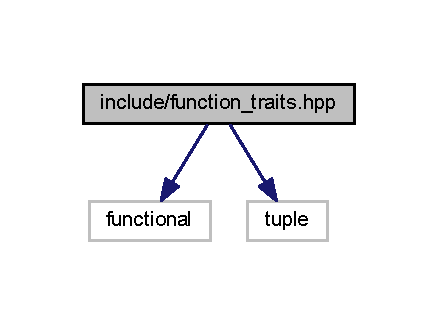
\includegraphics[width=210pt]{d3/d86/function__traits_8hpp__incl}
\end{center}
\end{figure}
\subsection*{Classes}
\begin{DoxyCompactItemize}
\item 
struct \hyperlink{structfn__traits_1_1function__traits}{fn\+\_\+traits\+::function\+\_\+traits$<$ Functor $>$}
\item 
struct \hyperlink{structfn__traits_1_1function__traits_3_01_r_07_args_8_8_8_08_4}{fn\+\_\+traits\+::function\+\_\+traits$<$ R(\+Args...)$>$}
\item 
struct \hyperlink{structfn__traits_1_1function__traits_3_01_r_07_args_8_8_8_08_4_d9/d01/structfn__traits_1_1function__traits_3_01_r_07_args_8_8_8_08_4_1_1arg}{fn\+\_\+traits\+::function\+\_\+traits$<$ R(\+Args...)$>$\+::arg$<$ i $>$}
\item 
struct \hyperlink{structfn__traits_1_1function__traits_3_01_r_07_5_08_07_args_8_8_8_08_4}{fn\+\_\+traits\+::function\+\_\+traits$<$ R($\ast$)(\+Args...)$>$}
\item 
struct \hyperlink{structfn__traits_1_1function__traits_3_01_r_07_c_1_1_5_08_07_args_8_8_8_08_4}{fn\+\_\+traits\+::function\+\_\+traits$<$ R(\+C\+::$\ast$)(\+Args...)$>$}
\item 
struct \hyperlink{structfn__traits_1_1function__traits_3_01_r_07_c_1_1_5_08_07_args_8_8_8_08_01const_01_01_4}{fn\+\_\+traits\+::function\+\_\+traits$<$ R(\+C\+::$\ast$)(\+Args...) const  $>$}
\item 
struct \hyperlink{structfn__traits_1_1function__traits_3_01_r_07_c_1_1_5_08_07_args_8_8_8_08_01volatile_01_4}{fn\+\_\+traits\+::function\+\_\+traits$<$ R(\+C\+::$\ast$)(\+Args...) volatile $>$}
\item 
struct \hyperlink{structfn__traits_1_1function__traits_3_01_r_07_c_1_1_5_08_07_args_8_8_8_08_01const_01volatile_01_4}{fn\+\_\+traits\+::function\+\_\+traits$<$ R(\+C\+::$\ast$)(\+Args...) const volatile $>$}
\item 
struct \hyperlink{structfn__traits_1_1function__traits_3_01std_1_1function_3_01_functor_01_4_01_4}{fn\+\_\+traits\+::function\+\_\+traits$<$ std\+::function$<$ Functor $>$ $>$}
\item 
struct \hyperlink{structfn__traits_1_1function__traits_3_01_t_01_6_01_4}{fn\+\_\+traits\+::function\+\_\+traits$<$ T \& $>$}
\item 
struct \hyperlink{structfn__traits_1_1function__traits_3_01const_01_t_01_6_01_4}{fn\+\_\+traits\+::function\+\_\+traits$<$ const T \& $>$}
\item 
struct \hyperlink{structfn__traits_1_1function__traits_3_01volatile_01_t_01_6_01_4}{fn\+\_\+traits\+::function\+\_\+traits$<$ volatile T \& $>$}
\item 
struct \hyperlink{structfn__traits_1_1function__traits_3_01const_01volatile_01_t_01_6_01_4}{fn\+\_\+traits\+::function\+\_\+traits$<$ const volatile T \& $>$}
\item 
struct \hyperlink{structfn__traits_1_1function__traits_3_01_t_01_6_6_01_4}{fn\+\_\+traits\+::function\+\_\+traits$<$ T \&\& $>$}
\item 
struct \hyperlink{structfn__traits_1_1function__traits_3_01const_01_t_01_6_6_01_4}{fn\+\_\+traits\+::function\+\_\+traits$<$ const T \&\& $>$}
\item 
struct \hyperlink{structfn__traits_1_1function__traits_3_01volatile_01_t_01_6_6_01_4}{fn\+\_\+traits\+::function\+\_\+traits$<$ volatile T \&\& $>$}
\item 
struct \hyperlink{structfn__traits_1_1function__traits_3_01const_01volatile_01_t_01_6_6_01_4}{fn\+\_\+traits\+::function\+\_\+traits$<$ const volatile T \&\& $>$}
\end{DoxyCompactItemize}
\subsection*{Namespaces}
\begin{DoxyCompactItemize}
\item 
 \hyperlink{namespacefn__traits}{fn\+\_\+traits}
\end{DoxyCompactItemize}
\subsection*{Typedefs}
\begin{DoxyCompactItemize}
\item 
{\footnotesize template$<$typename Functor $>$ }\\using \hyperlink{namespacefn__traits_adcf00e6412a39682ecf07be3958762f6}{fn\+\_\+traits\+::fn\+\_\+result\+\_\+of} = typename function\+\_\+traits$<$ Functor $>$\+::result\+\_\+type
\end{DoxyCompactItemize}


\subsection{Class Documentation}
\index{fn\+\_\+traits\+::function\+\_\+traits$<$ R(\+Args...)$>$\+::arg@{fn\+\_\+traits\+::function\+\_\+traits$<$ R(\+Args...)$>$\+::arg}}\label{structfn__traits_1_1function__traits_3_01_r_07_args_8_8_8_08_4_1_1arg}
\hypertarget{structfn__traits_1_1function__traits_3_01_r_07_args_8_8_8_08_4_structfn__traits_1_1function__traits_3_01_r_07_args_8_8_8_08_4_1_1arg}{}
\subsubsection{struct fn\+\_\+traits\+:\+:function\+\_\+traits$<$ R(Args...)$>$\+:\+:arg}
\subsubsection*{template$<$typename R, typename... Args$>$\\*
template$<$size\+\_\+t i$>$\\*
struct fn\+\_\+traits\+::function\+\_\+traits$<$ R(\+Args...)$>$\+::arg$<$ i $>$}



Definition at line 35 of file function\+\_\+traits.\+hpp.

\begin{DoxyFields}{Class Members}
typedef tuple\+\_\+element$<$ i, \\*
\hyperlink{structfn__traits_1_1function__traits_3_01_r_07_args_8_8_8_08_4_a9b60ae8c79e52addf352e4ae7c8077b4}{tuple\+\_\+type} $>$\+::\hyperlink{structfn__traits_1_1function__traits_3_01_r_07_args_8_8_8_08_4_ac0fde1bea9167cdc37a22b37bea78eb3}{type}\hypertarget{structfn__traits_1_1function__traits_3_01_r_07_args_8_8_8_08_4_ac0fde1bea9167cdc37a22b37bea78eb3}{}\label{structfn__traits_1_1function__traits_3_01_r_07_args_8_8_8_08_4_ac0fde1bea9167cdc37a22b37bea78eb3}
&
type&
\\
\hline

\end{DoxyFields}

\hypertarget{_r_e_a_d_m_e_8md}{}\section{R\+E\+A\+D\+M\+E.\+md File Reference}
\label{_r_e_a_d_m_e_8md}\index{R\+E\+A\+D\+M\+E.\+md@{R\+E\+A\+D\+M\+E.\+md}}

%--- End generated contents ---

% Index
\backmatter
\newpage
\phantomsection
\clearemptydoublepage
\addcontentsline{toc}{chapter}{Index}
\printindex

\end{document}
